%============================================================================
% tento soubor pouzijte jako zaklad
% (c) 2008 Michal Bidlo
% E-mail: bidlom AT fit vutbr cz
%============================================================================
% kodovaní: iso-8859-2 (zmena prikazem iconv, recode nebo cstocs)
%----------------------------------------------------------------------------
% zpracování: make, make pdf, make desky, make clean
% připomínky posílejte na e-mail: bidlom AT fit.vutbr.cz
% vim: set syntax=tex encoding=latin2:
%============================================================================
%\documentclass[cover]{fitthesis} % odevzdani do wisu - odkazy, na ktere se da klikat
\documentclass[print]{fitthesis} % pro tisk - na odkazy se neda klikat
%\documentclass[english,print]{fitthesis} % pro tisk - na odkazy se neda klikat
%      \documentclass[english]{fitthesis}
% * Je-li prace psana v anglickem jazyce, je zapotrebi u tridy pouzit 
%   parametr english nasledovne:
%      \documentclass[english]{fitthesis}
% * Neprejete-li si vysazet na prvni strane dokumentu desky, zruste 
%   parametr cover

% zde zvolime kodovani, ve kterem je napsan text prace
% "latin2" pro iso8859-2 nebo "cp1250" pro windows-1250, "utf8" pro "utf-8"
%\usepackage{ucs}
\usepackage[latin2]{inputenc}
\usepackage[T1, IL2]{fontenc}
\usepackage{url}
\DeclareUrlCommand\url{\def\UrlLeft{<}\def\UrlRight{>} \urlstyle{tt}}

%zde muzeme vlozit vlastni balicky
\graphicspath{{./fig/}}
\usepackage{amsmath}
\usepackage{mathtools}
\usepackage{listings}
\usepackage{graphicx}
\usepackage{color}
\usepackage{keystroke}
\usepackage{algorithmicx}
\usepackage{algpseudocode}
\usepackage{gensymb}
\definecolor{lightgray}{rgb}{.9,.9,.9}
\definecolor{white}{rgb}{1,1,1}
\definecolor{darkgray}{rgb}{.4,.4,.4}
\definecolor{purple}{rgb}{0.65, 0.12, 0.82}
\addto\captionsczech{\renewcommand{\figurename}{Diagram}}
%\renewcommand{\figurename}{Diagram}
\renewcommand{\lstlistingname}{Zdrojový kód}
\newcommand{\myparagraph}[1]{\paragraph{#1}\mbox{}\\}
\newcommand{\mysubparagraph}[1]{\subparagraph{#1}\mbox{}\\}


\lstdefinelanguage{JavaScript}{
  keywords={typeof, new, true, false, catch, function, return, null, catch, switch, var, if, in, while, do, else, case, break},
  keywordstyle=\color{blue}\bfseries,
  ndkeywords={class, export, boolean, throw, implements, import, this},
  ndkeywordstyle=\color{darkgray}\bfseries,
  identifierstyle=\color{black},
  sensitive=false,
  comment=[l]{//},
  morecomment=[s]{/*}{*/},
  commentstyle=\color{purple}\ttfamily,
  stringstyle=\color{red}\ttfamily,
  morestring=[b]',
  morestring=[b]"
}

\lstset{
   language=JavaScript,
   backgroundcolor=\color{lightgray},
   extendedchars=true,
   basicstyle=\footnotesize\ttfamily,
   showstringspaces=false,
   showspaces=false,
   numbers=left,
   numberstyle=\footnotesize,
   numbersep=9pt,
   tabsize=2,
   breaklines=true,
   showtabs=false,
   captionpos=b
}


% =======================================================================
% balíček "hyperref" vytváří klikací odkazy v pdf, pokud tedy použijeme pdflatex
% problém je, že balíček hyperref musí být uveden jako poslední, takže nemůže
% být v šabloně
\ifWis
\ifx\pdfoutput\undefined % nejedeme pod pdflatexem
\else
  \usepackage{color}
  \usepackage[unicode,colorlinks=false,hyperindex,plainpages=false,pdftex]{hyperref}
  \definecolor{links}{rgb}{0.4,0.5,0}
  \definecolor{anchors}{rgb}{1,0,0}
  \def\AnchorColor{anchors}
  \def\LinkColor{links}
  \def\pdfBorderAttrs{/Border [0 0 0] }  % bez okrajů kolem odkazů
  \pdfcompresslevel=9
\fi
\fi

%Informace o praci/projektu
%---------------------------------------------------------------------------
\projectinfo{
  %Prace
  project=BP,            %typ prace BP/SP/DP/DR
  year=2012,             %rok
  date={16. května 2012},           %datum odevzdani
  %Nazev prace
  title.cs={Implementace 3D logické hry v JavaScriptu},  %nazev prace v cestine
  title.en={Implementation of 3D Logic Game in JavaScript}, %nazev prace v anglictine
  %Autor
  author={Martin Knapovský},   %jmeno prijmeni autora
  %author.title.p=Bc., %titul pred jmenem (nepovinne)
  %author.title.a=PhD, %titul za jmenem (nepovinne)
  %Ustav
  department=UITS, % doplnte prislusnou zkratku: UPSY/UIFS/UITS/UPGM
  %Skolitel
  supervisor= Vendula Hrubá, %jmeno prijmeni skolitele
  supervisor.title.p=Ing.,   %titul pred jmenem (nepovinne)
  %supervisor.title.a={Ph.D.},    %titul za jmenem (nepovinne)
  %Klicova slova, abstrakty, prohlaseni a podekovani je mozne definovat 
  %bud pomoci nasledujicich parametru nebo pomoci vyhrazenych maker (viz dale)
  %===========================================================================
  %Klicova slova
  keywords.cs={JavaScript, WebGL, HTML5, Hra}, %klicova slova v ceskem jazyce
  keywords.en={JavaScript, WebGL, HTML5, Game}, %klicova slova v anglickem jazyce
  %Abstract
  abstract.cs={Tato bakalářská práce se zabývá vývojem logické webové hry, která vznikla na základě analýzy hry Berušky 2. Jsou zde stručně představeny technologie potřebně k vývoji a také teorie nutná k pochopení postupů použitých při implementaci. Výsledné řešení je podrobeno testům, jejichž výsledky jsou podkladem pro diskuzi obecné využitelnosti technologií, které se dnes v rámci webu nově objevují.}, % abstrakt v ceskem jazyce
  abstract.en={This bachelor's thesis describes development of a web game based on analysis of Berušky 2 game. Technologies needed for development are briefly introduced as well as the theory necessary for understanding the methods used in implementation. The final solution was put through tests, results of which serve as a basis for discussion about overall usability of technologies newly appearing on the web scene.}, % abstrakt v anglickem jazyce
  %Prohlaseni
  declaration={Prohlašuji, že jsem tuto bakalářskou práci vypracoval samostatně pod vedením paní Ing. Venduly Hrubé. Další informace mi poskytl pan Ing. Martin Stránský ze společnosti Red Hat. Uvedl jsem všechny literární prameny a publikace, ze kterých jsem čerpal.},
  %Podekovani (nepovinne)
  acknowledgment={Chtěl bych poděkovat paní Ing. Vendule Hrubé a panu Ing. Martinu Stránskému za jejich pomoc a rady při tvorbě této bakalářské práce.} % nepovinne
}

%Abstrakt (cesky, anglicky)
%\abstract[cs]{Tato bakalářská práce se zabývá vývojem 3D webové hry Berušky 2 WebGL a technologiemi k tomu potřebnými. Hra vznikla na základě analýzy hry Berušky 2, na jejímž vývoji se podílem pan Ing. Martin Stránský, který téma této práce vypsal.}
%\abstract[en]{This bachelor's thesis describes development of 3D web game Berušky 2 WebGL and used technologies. This game is based on anylisis of existing game Berušky 2, which was partly developed by Ing. Martin Stránský.}

%Klicova slova (cesky, anglicky)
%\keywords[cs]{Sem budou zapsána jednotlivá klíčová slova v českém jazyce, oddělená čárkami.}
%\keywords[en]{Sem budou zapsána jednotlivá klíčová slova v anglickém jazyce, oddělená čárkami.}

%Prohlaseni
%\declaration{Prohlašuji, že jsem tuto bakalářskou práci vypracoval samostatně pod vedením pana X...
%Další informace mi poskytli...
%Uvedl jsem všechny literární prameny a publikace, ze kterých jsem čerpal.}

%Podekovani (nepovinne)
%\acknowledgment{V této sekci je možno uvést poděkování vedoucímu práce a těm, kteří poskytli odbornou pomoc
%(externí zadavatel, konzultant, apod.).}

\begin{document}
  % Vysazeni titulnich stran
  % ----------------------------------------------
  \maketitle
  % Obsah
  % ----------------------------------------------
  \tableofcontents
  
  % Seznam obrazku a tabulek (pokud prace obsahuje velke mnozstvi obrazku, tak se to hodi)
  % \listoffigures
  % \listoftables 

  % Text prace
  % ----------------------------------------------
  \chapter{Úvod}
V dnešní době již webové technologie pokročily natolik, že je možné vytvářet takový obsah, který je plnohodnotnou aplikací s uživatelským rozhraním, multimediálním obsahem, či možností komunikace jejích uživatelů. Největší výhodou těchto aplikací je však to, že jsou dostupné komukoliv s kompatibilním webovým prohlížečem. Multiplatformnost aplikací tak není řešena tím, že bychom vytvářeli pro každý typ operačního systému příslušné spustitelné soubory, ale stačí pouze otevřít prohlížeč, zadat adresu a následně s aplikací pracovat. 
%Hra, jejíž vývoj je v této práci popisován tyto technologie využívá a je tedy možné ji používat na rozličných typech zařízení včetně moderních telefonů a tabletů.

Cílem této práce bylo navrhnout a implementovat logickou webovou hru založenou na hře Berušky 2 a ověřit tak vhodnost použití nově se objevujících technologií k tomutu účelu.

Technologie, jejich historie a použití jsou popsány v kapitole~\ref{chap:teorie}. Ta se primárně zaměřuje na WebGL, avšak jsou zde obsaženy i informace ohledně technologie HTML5, programovacího jazyka JavaScript a reprezentaci dat ve formátu JSON. V této kapitole je také obsažena teorie nutná k pochopení principů použitých při implementaci hry. Kapitola~\ref{chap:analysis} se zabývá analýzou původní hry Berušky 2, na jejímž základě je následně vypracován návrh implementované hry. Návrh webu, pomocí něhož je hra dostupná, je zmíněn pouze okrajově, jelikož není přímou součástí této práce. Implementační témata jsou obsažena v kapitole~\ref{chap:implementace} a testy výsledného řešení a jeho porovnání s původní hrou v kapitole~\ref{chap:testing}. Kapitola~\ref{chap:zaver} následně shrnuje poznatky získané při vývoji a diskutuje použitelnost technologií.

\chapter{Použité technologie a teorie}
V této kapitole jsou uvedeny informace týkající se technologií využítých při implementaci hry. Každá z nich je stručně představena a uvedena do souvislosti s touto prací. Mimo těchto informací kapitola také obsahuje teorii nutnou k pochopení postupů použitých při implementaci.

\label{chap:teorie}
\section{HTML5}
\label{section:html5}
HTML5\footnote{\url{http://www.w3.org/TR/html5/}} je připravovaným webovým standardem, který v první řadě vylepšuje podporu zobrazení multimediálního obsahu prostřednictvím webového prohlížeče. Co se týče doby od vydání předchozí specifikace HTML4.01\footnote{\url{http://www.w3.org/TR/REC-html40/}}, je nováčkem na poli webových technologií a jeho finální specifikace není v době psaní této práce stále dokončena. Vzhledem k tomu, že technologie  zahrnuté v jeho specifikaci řeší mnohé praktické problémy, vývojáři webových prohlížečů již nyní jednotlivé prvky HTML5 implementují. Experimenty s prohlížeči tak dávají pracovním skupinám spravujícím tuto specifikaci zpětnou vazbu, na jejímž základě lze provést mnohá vylepšení. Významnou vlastností specifikace je zpětná kompatibilita s její předchozí verzí, což umožňuje zobrazovat nové typy dokumentů v prohlížečích, které tyto technologie doposud neimplementují.~\cite{pilgrim2010html5, macdonald2011html5, lubbers2011pro}

Nejprve bude zmíněn historický vývoj a rozdělení HTML5 technologií, poté bude uveden výčet některých nových syntaktických a sémantických elementů, za nímž bude následovat popis elementu \texttt{<canvas>}, který je použit při implementaci hry.

\subsection*{Historie}
\label{subsection:historieHTML5}
Roku 2004 představili Mozilla Foundation a Opera Sorfware na W3C konzorciu návrh, který odrážel současné požadavky na webové aplikace. Tento návrh se soustředil na technologie, které by byly zpětně kompatibilní s tehdejšími webovými prohlížeči a zahrnoval také počáteční návrh specifikace Web Forms 2.0. Hlasování konzorcia dopadlo v neprospěch návrhu, což vedlo k tomu, že pracovní skupina W3C nadále soustředila své prostředky na vývoj specifikace XHTML2. Požadavky na webové aplikace však zůstaly nevyslyšeny, a tudíž byla hlavními představiteli vývojářů webových prohlížečů vytvořena nová pracovní skupina s názvem Web Hypertext Application Technology Working Group (WHATWG). O pět let později, roku 2009, zanechala W3C snahy protlačit specifikaci XHTML2 a spojila se s pracovní skupinou WHATWG, aby své usilí zaměřily na vývoj společného standardu HTML5.~\cite{pilgrim2010html5, macdonald2011html5, lubbers2011pro}

Značné popularity HTML5 nabylo po roce 2010, kdy tehdejší výkonný ředitel firmy Apple, Steve Jobs, prohlásil~\footnote{\url{https://www.apple.com/hotnews/thoughts-on-flash/}}, že na svých zařízeních nebudou nadále podporovat obsah zobrazovaný pomocí technologie Adobe Flash a zaměří se na podporu HTML5. Vzhledem k zastoupení této firmy na trhu začala valná většina velkých webových společností svůj obsah nabízet i pomocí této technologie.

V březnu roku 2011 vytyčila W3C cíle pro vývoj HTML5, kde určila rok 2014 jako cílový pro přijetí specifikace. Podmínky tohoto přijetí jsou 2 plně funkční implementace. Již dnes jsou mnohé implementace prvků stabilní a připraveny k použití. Jednou z nich je právě v implementaci hry využitý element \texttt{<canvas>}.


\subsection*{Rozdělení HTML5 technologií}
\label{subsection:rozdeleniHTML5}
Diagram technologií a jejich rozdělení je vyčleněn do přílohy~\ref{priloha:html5}. V následujících odstavcích jsou tyto kategorie stručně popsány. \\

\textbf{Oficiální W3C specifikace} zahrnuje nové syntaktické a sémantické elementy, nové a vylepšené web widgety, podporu pro audio/video a také element \texttt{<canvas>}, který slouží k vykreslování grafiky pomocí JavaScriptu. Tato část zahrnuje většinu prvků HTML5, které jsou prohlížeči dobře podporovány. 

\textbf{Prvky původního návrhu} patřily do specifikace, kterou připravila pracovní skupina WHATWG. Většina z nich vyžaduje ke své práci JavaScript a mezi ty nejdůležitější patří \textit{Local Data Storage} a \textit{Offline aplikace}. 

\textbf{Prky, které jsou často zahrnovány do HTML5} jsou například CSS3 a nástroje pro geolokaci.



\subsection*{Nové syntaktické a sémantické elementy HTML5}
\label{subsection:newElementsHTML5}
Nové sémantické elementy rozšiřují možnosti rozlišení úseků značkovaného textu. Na místě, kde byla typicky použita značka \texttt{<div>}, nebo \texttt{<span>} je nyní možné použít značky jako \texttt{<nav>} pro navigaci webu a dále pak například element \texttt{<footer>}, který označuje patičku dokumentu. 

\textbf{Video} a \textbf{audio} data byla v předchozích verzích HTML vkládána do dokumentů pomocí elementu \texttt{<object>}. Ten umožňoval označit obsah interpretovaný zásuvným modulem prohlížeče, kterým byl pro přehrávání videa nejčastěji Adobe Flash. Ten však díky novým možnostem HTML5 a přístupu firem jako Apple postupně ztrácí své dominantní postavení.

\pagebreak

\subsection*{Technologie HTML5 použité při implementaci}
\label{subsection:html5aImplementace}
Použité technologie:

\begin{itemize}
\item Canvas API\footnote{V textu lze často nalézt pojem API. API, neboli Applicaton Programming Interface je, jak z názvu vyplývá, rozhraní pro programování aplikací. Jedná se o sbírku procedur, funkcí, či tříd, které může programátor při tvorbě aplikace využívat.} 
\item WebGL
\item DOM API (Součást HTML5 Microdata)
\item Web Audio API
\end{itemize}

Z technologií HTML5 je při implementaci hry primárně využito \textbf{Canvas API}, které umožňuje prostřednictvím \textbf{WebGL} (podkapitola~\ref{section:webgl}) přistupovat k elementu \texttt{<canvas>} a vykreslovat tak 3D grafiku. \textbf{DOM API} je rozhraní pro přístup k prvkům zobrazovaného dokumentu a slouží k modifikaci jejich obsahu, struktury, nebo stylu, kterým jsou zobrazovány. \textbf{Web Audio API} je rozhraním elementu \texttt{<audio>}, které slouží k přehrávání herní hudby. Původní návrh hry zahrnoval také využítí technologie \textbf{localStorage}, která umožňuje uchovávat herní data na straně klienta bez nutnosti jejich načítaní při obnovení webové stránky. Vzhledem k tomu, že dnešní prohlížeče mají omezení na množství uložených dat\footnote{\url{http://dev-test.nemikor.com/web-storage/support-test/}}, nenalézá tato technologie v implementaci smysluplné využití. Na diagramu~\ref{priloha:html5} je také vyznačen JavaScriptový framework \textbf{jQuery}, jehož je využito hlavně pro vytvoření různých animací webu.

\subsection*{HTML5 \texttt{<canvas>}}
\label{subsection:HTML5canvas}
Základní HTML5 Canvas API obsahuje \textbf{2D} kontext, který umožňuje vykreslovat různé typy tvarů, text a také umožňuje zobrazovat obrazová data přímo do oblasti elementu \texttt{<canvas>}. Pro vykreslování je možné volit různé barvy, rotovat s prvky, zprůhledňovat je, či manipulovat s jednotlivými pixely tohoto elementu.

V souvislosti s WebGL mluvíme o \textbf{3D} kontextu, který umožňuje přímé vykreslování bitmapy, jejíž obsah je možné měnit pomocí JavaScriptu. U 3D kontextu je při každém volání vykreslovacího rozhraní plocha elementu zcela překreslena a je tedy programátorovou prací připravit vykreslovaný obraz před každým voláním. Tím se \texttt{<canvas>} odlišuje od technologií jako Flash, Silverlight, nebo SVG, které vykreslovaný obraz pouze aktualizují (umožňují například posouvat vykreslované objekty scény vůči své aktuální pozici), což na jednu stranu programátora odstiňuje od nízkoúrovňových operací, avšak na stranu druhou má programátor omezenou kontrolu nad výsledným vykresleným obrazem. Podrobnější informace o tom, jak vykreslování pracuje jsou součástí podkapitoly~\ref{section:webgl}.

\pagebreak

\section{Javascript}
\label{section:javascript}
Většina webových stránek se dnes podobá plnohodnotným desktopovým aplikacím právě díky JavaScriptu. JavaScript je programovací jazyk, který umožňuje vylepšit zobrazovaný dokument prostřednictvím animací, interaktivitou, nebo dynamickými visuálními efekty. Jeho velkou výhodou je to, že stránky reagují na podněty uživatele okamžitě - při vyplňování formuláře, nebo v moment, kdy uživatel pohne myší na určitou pozici. Jeho zpracování je totiž oproti jiným skriptovacím jazykům používaným na webu prováděno na klientském zařízení (avšak nejen tam, jak bude uvedeno dále). V současné době je jeho masivní využití vidět v projektech jako Facebook\footnote{\url{www.facebook.com}}, nebo například Google Maps\footnote{\url{maps.google.com}}.

Popularita tohoto jazyka roste a s ním i jeho využití. Nejen, že jeho interprety lze dnes nalézt ve všech webových prohlížečích na stolních počítačích, herních konzolích, chytrých telefonech či tabletech, ale je využit také pro popis grafických rozhraní desktopových aplikací, nebo jako jazyk použitý na straně serveru. Příklady využití JavaScriptu mimo web jsou uvedeny v následujícím přehledu.

\begin{itemize}
\item Doplňky pro prohlížeč Google Chrome, Opera, Safari
\item Apple dashboard widgety
\item JavaScript v pdf souborech
\item Skriptování v Adobe Photoshop, Illustrator, InDesign
\item Zpracování signálu v Max/MSP pro program Ableton Live
\item Skriptování v Unity
\item JavaScript v prostředí Javy
\item Popis grafického rozhraní v knihovně Qt
\item \ldots
\end{itemize}

\subsection*{Historie jazyka}
\label{subsection:jsHistorie}
Autorem jazyka je Brendan Eich z tehdejší společnosti Netscape. Jazyk byl nejdříve vyvíjen pod názvem \textit{\uv{Mocha, LiveScript}}, avšak s vydáním prohlížeče Netscape 2.0B3, jehož byl tento jazyk součástí, se název z marketingových důvodů změnil na JavaScript. Jeho velký úspěch vedl k tomu, že společnost Microsoft vytvořila jeho obdobu pro svůj prohlížeč Internet Explorer, kterou nazvala JScript. V roce 1997 byl jazyk standardizován pod názvem ECMAScript, ze kterého byly následně odvozeny i další implementace, jako je například ActionScript. Svého největšího rozmachu se tento jazyk dočkal s rozšířením technik, které se souhrnně označují jako AJAX (\ref{subsection:AJAX}).\cite{flanagan2006javascript}

\subsection*{Stručný popis jazyka JavaScript}
\label{subsection:jsPopis}
JavaScript je multiplatformní, dynamický, slabě typovaný skriptovací jazyk. Podporuje různá paradigmata včetně objektového, čehož je v implementaci hry často využíváno. Syntaxe jazyka je ovlivněna konvencemi jazyků Java a C, principiálně je však jazyk vystavěn podobně jako jazyky Self a Scheme. Způsob, jakým jsou vytvářeny objekty, je zde oproti klasickým jazykům jako C++ nebo Java odlišný díky tomu, že je tento jazyk prototypově založený. Třídy jsou tak nahrazeny konstruktory objektů a dědičnost prototypováním.\cite{flanagan2006javascript} Příklad vytvoření konstruktoru objektu a jeho následné použití je uveden ve zdrojovém kódu~\ref{code:jsObjectConstructor}.
%\medskip
\begin{lstlisting}[caption=Příklad vytvoření objektu v JavaScriptu,label=code:jsObjectConstructor]
function TestObject(num){

    this.property1 = 1;
    this.property2 = this.property1;
    this.property3 = num;
}

var test = new TestObject(5);
alert(test.property1); // 1
alert(test.property2); // 1
alert(test.property3); // 5

test.property1 = 6;
alert(test.property1); // 6
\end{lstlisting}

JavaScript interaguje s webovou stránkou prostřednictvím dříve popsaného rozhraní DOM tak, že se naváže zpracování událostí vytvářených uživatelem na funkce, které je zpracovávají. Rozhraní DOM však není přesně standardizované a prohlížeče ho implementují různě. U některých prvků je tedy nutné rozlišovat, který prohlížeč JavaScript aktuálně interpretuje a dle toho volit, jakým způsobem se s nimi bude nakládat. Jako příklad je ve zdrojovém kódu~\ref{code:jsMouseEvent} uvedeno zpracování události pohybu kolečka myši.

\begin{lstlisting}[caption=Zpracování události pohybu kolečka myši,label=code:jsMouseEvent]
function handleWheel(event) {
    var delta = 0;
    
    // Zpracování události v Internet Exploreru
    if (!event){
       event = window.event;
    }
	
		// Internet Explorer, Opera, Chrome
		if (event.wheelDelta) {
	    	delta = event.wheelDelta / 120;
		}
		// Mozilla Firefox
		else if (event.detail) {
	    	delta = -event.detail / 3;
		}
    // ...
}
\end{lstlisting}

\subsection*{AJAX}
\label{subsection:AJAX}
AJAX, neboli Asynchronous JavaScript and XML, je souhrnné označení pro vzájemně propojené techniky používané na klientské straně webových aplikací. Tyto techniky umožňují asynchronně nahrát data ze serveru, což pro uživatele znamená, že aktuálně zobrazená webová stránka nemusí být znovu načtena a interakce s aplikací je tak mnohem přívětivější. Využívá se přitom \texttt{XMLHttpRequest} objektu, který je dostupný prostřednictvím JavaScriptu. Navzdory názvu, který vyzdvihuje přenos dat ve formátu XML, je možné použít i formáty jiné. Ve hře je těchto technik využito k načtení herních úrovní, které jsou reprezentovány soubory formátu JSON a následně pak potřebných textur a lightmap. 

%diagram AJAX

\subsection*{JavaScript Frameworky}
\label{subsection:jsFrameworky}
JavaScriptové frameworky slouží k urychlenému vývoji webových aplikací. Vytvářejí jakousi vrstvu nad základními prostředky jazyka a poskytují k nim tak zjednodušený přístup. Frameworků pro jazyk JavaScript existuje celá řada, avšak pro implementaci bylo využito jednoho z nejznámějších - jQuery.

jQuery umožňuje přistupovat k prvkům DOM tak, že se rozdíly mezi prohlížeči (jako třeba právě zpracování události kolečka myši) stírají a k prvkům je tak přistupováno jednotnou formou. Za základě událostí generovaných uživatelem je také umožněno animovat vzhled prvků dokumentu - měnit jejich pozice, průhlednost, či například vrstvu, ve které se mají zobrazit. Toho je ve hře využito velmi často, avšak vzhledem k tomu, že se jedná o animace webu samotného, který není přímou součástí této práce, nebude jejich popisu věnováno mnoho prostoru. Příklad animace průhlednosti prvku je uveden ve zdrojovém kódu~\ref{code:jsAnimation}.

\begin{lstlisting}[caption=jQuery Animace,label=code:jsAnimation]
// Animace průhlednosti z aktuální hodnoty na hodnotu 0.0 za čas 1000 ms.
// Po dokončení animace je zavolána anonymní funkce měnící vrstvu,
// ve které se prvek zobrazuje.
$("#item").animate({'opacity':'0.0'}, 1000, function(){
    $("#item").css({'z-index':'-1'});
});
\end{lstlisting}

\section{JSON}
\label{section:JSON}
JSON, neboli JavaScript Object Notation je otevřený standard určený pro výměnu dat. Jeho notace je odvozena od JavaScriptu, což oproti dalšímu rozšířenému formátu pro přenos dat - XML, usnadňuje práci s daty v tomto programovacím jazyku. XML dokáže svým značkováním lépe popsat kontext toho, co přenáší, avšak za cenu většího objemu dat. Proto je také JSON chápán jako odlehčená verze XML. JSON není použit pouze v programovacím jazyku JavaScript, avšak v dnešní době můžeme nalézt jeho syntaktické analyzátory i v knihovnách mnohých dalších jazyků.\cite{flanagan2006javascript} \\ \\
JSON je založen na dvou strukturách:
\begin{itemize}
\item Kolekce párů název/hodnota. Ta bývá v rozličných jazycích realizována jako objekt, záznam (record), struktura (struct), slovník (dictionary), hash tabulka, klíčový seznam (keyed list), nebo asociativní pole.
\item Tříděný seznam hodnot. Ten je ve většině jazyků realizován jako pole, vektor, seznam (list) nebo posloupnost (sequence).
\end{itemize}

Na následujících diagramech je znázorněna JSON syntaxe zápisu objektu (\figurename\ \ref{fig:jsonObject}), pole (\figurename\ \ref{fig:jsonArray}) a hodnoty (\figurename\ \ref{fig:jsonValue}).

\begin{figure}[htb]
\centering
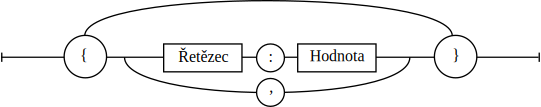
\includegraphics[width=0.8\textwidth]{jsonObject}
\caption{JSON Objekt}
\label{fig:jsonObject}
\end{figure}

\begin{figure}[htb]
\centering
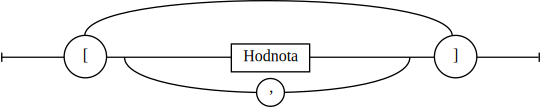
\includegraphics[width=0.8\textwidth]{jsonArray}
\caption{JSON Pole}
\label{fig:jsonArray}
\end{figure}

\begin{figure}[htb]
\centering
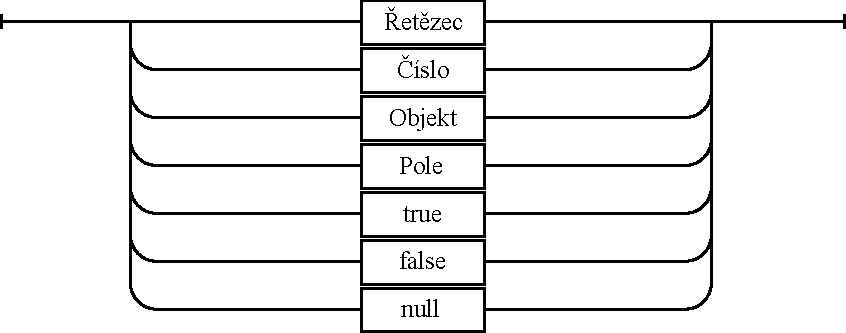
\includegraphics[width=0.8\textwidth]{jsonValue}
\caption{JSON Hodnota}
\label{fig:jsonValue}
\end{figure}

JSON je ve hře použit pro reprezentaci herních úrovní. Vzhledem k tomu, že při použití jakéhokoliv jiného formátu by bylo potřeba na vstupu provádět jeho parsování, což by hru zbytečně zpomalovalo, je tento formát v podstatě jediným vhodným kandidátem.

\section{Lineární algebra pro 3D grafiku}
\label{section:linearniAlgebra}
Lineární algebra je ta část matematiky, která se zabývá vektory a maticemi. Pro porozumění 3D grafice a WebGL je dobré mít alespoň základní znalosti v tomto oboru. Vzhledem k rozsahu této práce není možné zmínit vše, a proto jsou pojmy jako souřadný systém, vektory a jejich skalární a vektorový součin považovány za znalost čtenáře. Následující text se soustředí na homogenní souřadnice, matice a transformace ve 3D grafice.

\subsection*{Homogenní souřadnice}
\label{subsection:homogenniSouradnice}
V 3D prostoru je možné bod\footnote{Ve 3D grafice nazývaný \textit{vertex}} definovat pomocí tří souřadnic. To však může být matoucí v tom, že body a vektory jsou definovány stejným způsobem. S homogenními souřadnicemi přidáváme čtvrtou souřadnici, která je značena jako \textit{w}. Pro vektory je pak $w=0$, a pokud je $w!=0$, pak homogenní souřadnice definují bod. Homogenní bod lze převést na tříprvkový bod vydělením všech souřadnic souřadnicí homogenní. Pro převod tříprvkového bodu na bod homogenní pak stačí přidat jako homogenní souřadnici hodnotu 1. Homogenní souřadnice se používají z toho důvodu, že ve 3D grafice jsou nejčastější operací různé transformace, které jsou popsány pomocí $4\times4$ matic. Abychom mohli bod pomocí těchto matic transformovat, je nutné, aby byl bod popsán právě čtyřmi souřadnicemi.

\subsection*{Matice}
\label{subsection:matice}
Matice je složena z řádků a sloupců. Elementy uvnitř matice se nazývají prvky matice a dle počtu řádků a sloupců rozlišujeme různé její dimenze. Nejčastěji používaným typem jsou ve WebGL matice se čtyřmi řádky a čtyřmi sloupci. Tyto pak označujeme jako $4\times4$ matice.

\begin{equation}
 M = \begin{bmatrix}
       m_{00} & m_{01} & m_{02} & m_{03}     \\[0.3em]
       m_{10} & m_{11} & m_{12} & m_{13}     \\[0.3em]
       m_{20} & m_{21} & m_{22} & m_{23}     \\[0.3em]
       m_{30} & m_{31} & m_{32} & m_{33}     \\[0.3em]
     \end{bmatrix}
\end{equation}

Maticím s jedním sloupcem ($m \times 1$) se také jinak říká sloupcový vektor a maticím s jedním řádkem řádkový vektor ($1 \times m$).

\begin{align}
%\begin{split}
 V = \begin{bmatrix}
       v_{0} \\[0.3em]
       v_{1} \\[0.3em]
       v_{2} \\[0.3em]
       v_{3} \\[0.3em]
     \end{bmatrix} \\
%\end{split}
%\begin{split}
V = \begin{bmatrix}
       v_{0} & v_{1} & v_{2} & v_{3}  \\[0.3em]
     \end{bmatrix}
%\end{split}\tag{2.2a, 2.2b} 
\end{align}
%\tag{1a,b} 

\myparagraph{Součet a rozdíl matic}
Součet a rozdíl je možný, pokud mají matice stejné dimenze. Součet, nebo rozdíl pak probíhá prvek po prvku.


\begin{align}
%\begin{split}
 A = \begin{bmatrix}
       1 & 5 & 3 \\[0.3em]
       4 & 4 & 1 \\[0.3em]
     \end{bmatrix} \\
%\end{split}
%\begin{split}
 B = \begin{bmatrix}
       5 & 3 & 3 \\[0.3em]
       2 & 5 & 2 \\[0.3em]
     \end{bmatrix} \\
%\end{split}\tag{2.3a, 2.3b} 
%\end{align}
%\begin{align}
 A + B = \begin{bmatrix}
       6 & 8 & 6 \\[0.3em]
       6 & 9 & 3 \\[0.3em]
     \end{bmatrix}
\end{align}

\myparagraph{Násobení matic}
Násobení matic je ve 3D grafice velmi důležitou operací. Definice násobení je taková, že dvě matice mohou být vzájemně vynásobeny pouze tehdy, když se počet sloupců první matice rovná počtu řádků matice druhé. Výsledná matice má pak počet řádků rovný matici první a počet sloupců matici druhé.

\begin{align}
[m \times p][p \times n] = [m \times n]
\end{align}

Prvky \textit{ij} výsledné matice vzniknou skalárním vynásobením řádku \textit{i} matice \textbf{A} a sloupce \textit{j} matice \textbf{B}.

\begin{align}
M = 
\begin{bmatrix*}[r]
  -3 & 1 \\
  -2 & 2 \\
  -4 & 5 \\
\end{bmatrix*} \\
N =
\begin{bmatrix*}[r]
  -4 & 3 \\
   3 & 5 \\
\end{bmatrix*}
\end{align} 
\begin{align}
M \times N = 
\begin{bmatrix*}[r]
  (-3) \times (-4) + 1 \times 3 & (-3) \times 3 + 1 \times 5 \\
  (-2) \times (-4) + 2 \times 3 & (-2) \times 3 + 2 \times 5 \\
  (-4) \times (-4) + 5 \times 3 & (-4) \times 3 + 5 \times 5 \\
\end{bmatrix*}
=
\begin{bmatrix*}[r]
  15 & -4 \\
  14 & 4 \\
  31 & 13 \\
\end{bmatrix*}
\end{align}


\myparagraph{Matice identity a inverzní matice}
Matice identity je takovou maticí, že pokud s ní vynásobíme jakoukoliv matici jinou, tak získáme opět tu samou.

\begin{align}
M \times I = I \times M = M
\end{align}

Matice identity je vždy čtvercová (stejný počet sloupců jako řádků), na své diagonále má prvky rovny 1 a mimo diagonálu 0.

\begin{align}
I = 
\begin{bmatrix*}[r]
  1 & 0 & 0 & 0 \\
  0 & 1 & 0 & 0 \\
  0 & 0 & 1 & 0 \\
  0 & 0 & 0 & 1 \\
\end{bmatrix*}
\end{align}

Nyní, když víme, co je to matice identity, můžeme přistoupit k definici matice inverzní. Pro jakékoliv číslo $x$ (kromě 0) nalezneme číslo $1/x$ (zapisováno také jako $x^{-1}$), které při vynásobení touto inverzní hodnotou dává jako svůj výsledek hodnotu 1. Podobně je definována i matice inverzní, kterou označujeme jako $M^{-1}$.

\begin{align}
M \times M^{-1} = M^{-1} \times M = 1
\end{align}

Je důležité poznamenat, že pouze čtvercové matice mají matici inverzní.

\myparagraph{Transponovaná matice}
Transponovaná matice vznikne prohozením svých řádků se sloupci. Matice je definována pro jakékoliv dimenze a označuje se jako $M^{T}$. Vzhledem k tomu, že ve WebGL se používají matice $4\times4$, jsou i zde příklady uvedeny v těchto dimenzích.

\begin{align}
 M = 
\begin{bmatrix*}[r]
  1 & 2 & 3 & 4 \\
  5 & 6 & 7 & 8 \\
  9 & 10 & 11 & 12 \\
  13 & 14 & 15 & 16 \\
\end{bmatrix*}
\end{align}

\begin{align} 
M^T = 
\begin{bmatrix*}[r]
  1 & 5 & 9 & 13 \\
  2 & 6 & 10 & 14 \\
  3 & 7 & 11 & 15 \\
  4 & 8 & 12 & 16 \\
\end{bmatrix*}
\end{align}

\subsection*{Transformace}
\label{subsection:transformace}
Transformace je operace, která na svém vstupu přijímá jakousi entitu, jakou je například bod, nebo vektor, a nějakým způsobem ji modifikuje. Speciálním typem transformace je pak transformace lineární, což je zobrazení $f$ z jednoho vektorového prostoru do druhého $f: V \rightarrow W$, které zachovává vektorové operace sčítání a násobení skalárem. Název \textit{lineární} je odvozen z faktu, že grafem obecného lineárního zobrazení z reálných čísel do reálných čísel je přímka.

Mějme dva vektory $u$, $v$ a transformaci reprezentovanou pomocí funkce $f$. Pak lineární transformací je operace, která splňuje následující podmínky:

\begin{align}
\begin{split}
f(u) + f(v) = f(u+v) 
\end{split}
\begin{split}
 (aditivita)
\end{split} \\
\begin{split}
kf(u) = f(ku)
\end{split}
\begin{split}
 (homogenita)
 \end{split}
\end{align}


Mezi lineární transformace patří například posunutí (translace), rotace, změna měřítka (scaling), či zkosení (shearing). Násobením transformačních matic lze vytvářet ze základních transformací transformace komplexní. Při násobení však musíme dávat pozor na pořadí, ve kterém jsou matice násobeny. Násobení matic totiž není komutativní operací. Jakákoliv transformace bodu, nebo vektoru v 3D prostoru může být vyjádřena pomocí $4 \times 4$ matice.

\begin{align} 
Mv = \begin{bmatrix*}[r]
  m_{00} & m_{01} & m_{02} & m_{03} \\
  m_{10} & m_{11} & m_{12} & m_{13} \\
  m_{20} & m_{21} & m_{22} & m_{23} \\
  m_{30} & m_{31} & m_{32} & m_{33} \\
\end{bmatrix*}
\begin{bmatrix*}[r]
 v_{0} \\
 v_{1} \\
 v_{2} \\
 v_{3} \\
\end{bmatrix*} =
\begin{bmatrix*}[r]
  m_{00}v_{0} & m_{01}v_{1} & m_{02}v_{2} & m_{03}v_{3} \\
  m_{10}v_{0} & m_{11}v_{1} & m_{12}v_{2} & m_{13}v_{3} \\
  m_{20}v_{0} & m_{21}v_{1} & m_{22}v_{2} & m_{23}v_{3} \\
  m_{30}v_{0} & m_{31}v_{1} & m_{32}v_{2} & m_{33}v_{3} \\
\end{bmatrix*}
\end{align}

\pagebreak
\myparagraph{Translace}
Translace je lineární transformací, která posouvá bod v prostoru. Translační matice vypadá následovně:

\begin{align}
T(t_x, t_y, t_z) = 
\begin{bmatrix*}[r]
 1 & 0 & 0 & t_x \\
 0 & 1 & 0 & t_y \\
 0 & 0 & 1 & t_z \\
 0 & 0 & 0 & 1 \\
\end{bmatrix*}
\end{align}

Uvedená translační matice posouvá bod s ofsetem, který je reprezentován pomocí vektoru $(t_x, t_y, t_z)$. Diagram~\ref{fig:translation} znázorňuje translaci bodů krychle násobením s následující maticí:

\begin{align}
T(4, 5, 0) = 
\begin{bmatrix*}
1 & 0 & 0 & 5 \\
0 & 1 & 0 & 0 \\
0 & 0 & 1 & 0 \\
0 & 0 & 0 & 1 \\
\end{bmatrix*}
\end{align}

\begin{figure}[htb]
\centering
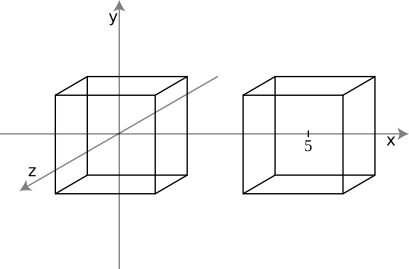
\includegraphics[width=0.8\textwidth]{translation}
\caption{Translace}
\label{fig:translation}
\end{figure}


\subsection*{Rotace}
Tato transformace rotuje bod, či vektor o zadaný úhel kolem počátku souřadného systému $[0, 0, 0]$. Běžně se používají rotační matice pro rotaci kolem osy\footnote{Rotace se řídí tzv. pravidlem pravé ruky. Palec směřuje v kladném směru osy a zbylé zatočené prsty ruky naznačují směr kladné rotace.} x, y a z. 

\begin{align}
R_x(\phi) = 
\begin{bmatrix*}
1 & 0 & 0 & 0 \\
0 & \cos\phi & -\sin\phi & 0 \\
0 & \sin\phi & \cos\phi & 0 \\
0 & 0 & 0 & 1 \\
\end{bmatrix*}
\end{align}

\begin{align}
R_y(\phi) = 
\begin{bmatrix*}
\cos\phi & 0 & \sin\phi & 0 \\
0 & 1 & 0 & 0 \\
-\sin\phi & 0 & \cos\phi & 0 \\
0 & 0 & 0 & 1 \\
\end{bmatrix*}
\end{align}

\begin{align}
R_z(\phi) = 
\begin{bmatrix*}
\cos\phi & -\sin\phi & 0 & 0 \\
\sin\phi & \cos\phi & 0 & 0 \\
0 & 0 & 1 & 0 \\
0 & 0 & 0 & 1 \\
\end{bmatrix*}
\end{align}

Diagram~\ref{fig:rotation} znázorňuje rotaci bodů krychle kolem počátku soustavy souřadnic s využitím této transformační matice:

\begin{align}
R_x(30^{\circ}) = 
\begin{bmatrix*}
1 & 0 & 0 & 0 \\
0 & \cos(30^{\circ}) & -\sin(30^{\circ}) & 0 \\
0 & \sin(30^{\circ}) & \cos(30^{\circ}) & 0 \\
0 & 0 & 0 & 1 \\
\end{bmatrix*}
\end{align}

\begin{figure}[htb]
\centering
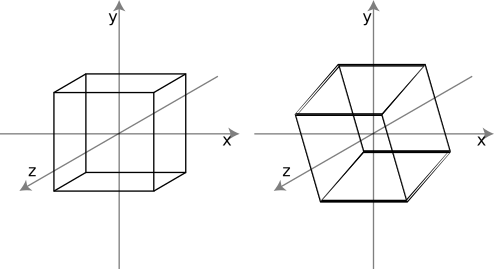
\includegraphics[width=0.8\textwidth]{rotation}
\caption{Rotace}
\label{fig:rotation}
\end{figure}

Dalšími transformacemi používanými ve 3D grafice je tzv. scaling, který zvětšuje, či zmenšuje objekt a pak tzv. shearing, který dokáže objekt zkosit dle dané osy. Tyto dvě transformace však nejsou při implementaci hry využity, a tudíž zde nebudou zmíněny.

\pagebreak
\section{WebGL}
\label{section:webgl}
WebGL je nízkoúrovňové aplikační rozhraní pro zobrazení pokročilé 3D grafiky na webu. Je založeno na OpenGL ES 2.0 a umožňuje programátorovi použít hardwarově akcelerované\footnote{K hardwarové akceleraci je nutno vlastnit GPU s podporou minimálně shader modelu 2.0. V opačném případě lze obraz vykreslovat softwarově.} vykreslování obrazu v kontextu HTML a JavaScriptu. Vykreslovací plochou, která je zde použita je HTML5 \texttt{<canvas>} element a jeho \texttt{webgl}, resp. \texttt{experimental-webgl} kontext.~\cite{seidelin2011html5}

\subsection*{Historie WebGL}
\label{subsection:historieWebGL}
První experimenty s 3D grafikou v \texttt{<canvas>} elementu prováděl Vladimir Vukićević ze společnosti Mozilla. Výsledkem jeho pokusů se stal prototyp, který nazval Canvas 3D. V roce 2009 vytvořila Khronos Group novou pracovní skupinu pro WebGL, která byla složena z hlavních tvůrců webových prohlížečů včetně firem jako Apple, Google, Mozilla a Opera. Khronos Group je neziskovou organizací, která vytváří a spravuje otevřené standardy a aplikační rozhraní. Byla založena roku 2000 a mimo jiné stojí i za standardy jako OpenGL, či výše zmíněným OpenGL ES, které je primárně určeno pro vestavěné systémy.~\cite{anyuru2012professional}

Finální specifikace WebGL 1.0\footnote{\url{http://www.khronos.org/registry/webgl/specs/1.0/}} byla vydána v březnu roku 2011 a její implementaci můžeme nalézt v prohlížečích jako Google Chrome, Mozilla Firefox, Safari a v počátečních fázích implementace v prohlížeči Opera. V případě Microsoft Internet Exploreru je situace poněkud odlišná. Microsoft neohlásil žádný záměr v podpoře WebGL ve svém prohlížeči. Uživatelé, kteří chtějí WebGL používat, jsou tedy nuceni přejít k jinému prohlížeči.~\cite{anyuru2012professional}

\subsection*{Výhody WebGL}
\label{subsection:vyhodyWebGL}
V dobách, kdy web jako takový začínal, byl jeho obsah vytvořen ze statických dokumentů. Hlavní prací webových prohlížečů tehdy bylo takovýto obsah získat a zobrazit. V průběhu času však webové technologie značně pokročily a nyní tak jejich prostřednictvím mužeme přistupovat k plnohodnotným webovým aplikacím s bohatým uživatelským rozhraním a audiovizuálním obsahem. Tyto aplikace se nyní stávají alternativou k aplikacím nativním.~\cite{anyuru2012professional} \\ \\
Jejich hlavními výhodami jsou:
\begin{itemize}
\item Rychlá \textbf{dostupnost} a jednoduchá \textbf{distribuce} mezi mnoho uživatelů.
\item \textbf{Snadná údržba a aktualizace aplikací.} Pokud je v aplikaci nalezena chyba, nebo pokud chceme rozšířit její funkcionalitu, pak vše, co je potřeba, je aktualizovat aplikaci na serveru a uživatelé mají ihned přístup k její nové verzi.
\item \textbf{Multiplatformnost aplikací.} Vše, co uživatel potřebuje je kompatibilní webový prohlížeč schopný zobrazit námi definovaný obsah.
\end{itemize}

Oproti nativním aplikacím nejsou ty webové obsahem tak bohaté, avšak s příchodem HTML5 začíná tento rozdíl mizet. Prostřednictvím WebGL je nyní možné zobrazovat hardwarově akcelerovanou grafiku přímo uvnitř prohlížeče. Je tak možné vytvořit 3D hry, nebo pokročilé 3D grafické aplikace a zároveň těžit z výhod webu, jak byli popsány výše. Technologie WebGL má navíc i další výhody, mezi něž patří například:
\begin{itemize}
\item WebGL je otevřený standard, který může používat každý bez poplatků.
\item WebGL využívá přímo grafický hardware, což znamená, že jsou aplikace rychlé.
\item Vzhledem k tomu, že je WebGL založeno na OpenGL ES, je možné vytvořené aplikace spouštět i na mnohých moderních mobilních zařízeních.
\end{itemize}

\subsubsection*{Grafická API}
\label{subsection:grafickaAPI}
Existují dva fundamentální přístupy, které jsou u grafických aplikačních rozhraní využity. Jsou jimi:
\begin{itemize}
\item immediate-mode API a 
\item retained-mode API,
\end{itemize}
přičemž WebGL používá první ze zmíněných přístupů.


\myparagraph{Immediate-mode API} 
U tohoto typu rozhraní je celá scéna překreslena s každým snímkem bez ohledu na to, zda byla změněna, či nikoliv. Grafická knihovna která zprostředkovává rozhraní programátorovi neukládá žádnou interní reprezentaci scény, která má být vykreslena. Reprezentaci scény je tak nutné uchovávat v paměti vlastní aplikace. Tento přístup je vysoce flexibilní a poskytuje programátorovi větší úroveň kontroly nad výsledným vykreslovaným obrazem. Na druhou stranu však tento přístup vyžaduje ze strany programátora více úsilí oproti přístupu, který si popíšeme nyní.

\begin{figure}[htb]
\centering
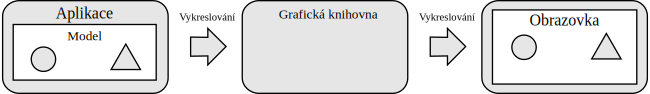
\includegraphics[width=0.8\textwidth]{immediateMode}
\caption{Immediate-mode API}
\label{fig:immediateMode}
\end{figure}

\myparagraph{Retained-mode API} 
U tohoto přístupu je interní model a veškeré vykreslované objekty scény obsažen v grafické knihovně, která toto rozhraní programátorovi nabízí. Programátor využívá přístupových metod k rozhraní a knihovna sama rozhoduje o tom, zda má být scéna a s ní její interní reprezentace aktualizována, či nikoliv. To znamená, že aplikace, která rozhraní využívá, nemusí v každém vykreslovaném snímku scénu překreslovat. Tento přístup je v mnohých ohledech pro programátora méně náročný a používá se například pro vykreslování vektorové grafiky (SVG). 

\begin{figure}[htb]
\centering
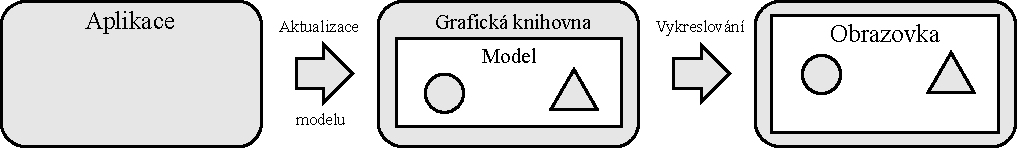
\includegraphics[width=0.8\textwidth]{retainedMode}
\caption{Retained-mode API}
\label{fig:retainedMode}
\end{figure}
 
\subsection*{Tvorba obrazu v grafickém hardwaru}
\label{subsection:tvorbaObrazu}
WebGL je nízkoúrovňové rozhraní a pracuje tak velmi blízko grafického hardwaru. K pochopení fundamentálních konceptů použitých při implementaci hry je tedy nejprve potřeba alespoň okrajově osvětlit, jakým způsobem grafický hardware pracuje. 

Na diagramu~\ref{fig:gpuDisplay} je zjednodušeně znázorněn vztah grafického hardwaru k ostatním částem systému.

\begin{figure}[htb]
\centering
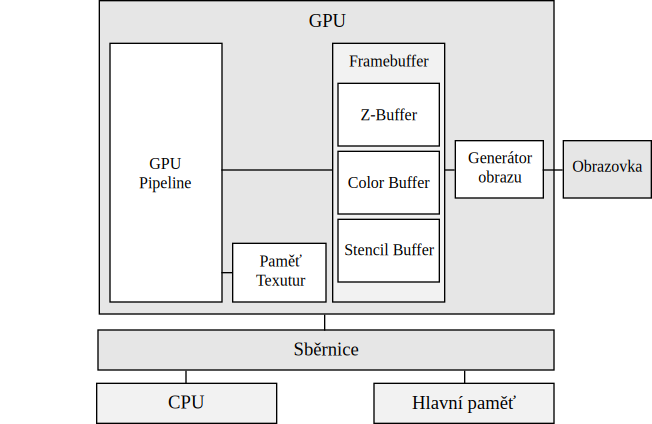
\includegraphics[width=0.8\textwidth]{gpuDisplay}
\caption{Vztah grafického hardwaru k ostatním částem systému}
\label{fig:gpuDisplay}
\end{figure}

\myparagraph{GPU}
GPU, neboli také Graphics Processing Unit, je dedikované zařízení, které je přímo navrženo pro zobrazení grafiky. Architektura GPU je vysoce paralelizovaná a provádí operace s grafickými daty velmi rychle. Zpracování dat probíhá typicky zřetězeně v několika úrovních.

\myparagraph{Framebuffer}
Framebuffer je místem, kde je uložen výsledek operací provedených na GPU. Je to paměť, která obsahuje informace nutné pro zobrazení výsledného obrazu na zobrazovací zařízení. V jednoduchém grafickém systému může být fyzická paměť framebufferu součástí hlavní operační paměti, avšak u moderních systémů je tato paměť alokována ve speciální rychlé grafické paměti na GPU. Framebuffer se typicky skládá ze tří odlišných \textit{subbufferů}.

\begin{itemize}
\item Color Buffer
\item Z-Buffer
\item Stencil Buffer
\end{itemize}

\mysubparagraph{Color Buffer}
Color buffer představuje dvourozměrné pole, jehož prvky jsou výsledné barvy pixelů obrazu. Každý z těchto prvků obsahuje informaci o výsledné barvě v RGB, či RGBA formátu. Každý z barevných kanálů má alokován určitý počet bitů a navíc může být obsažena informace o \textit{alpha} kanálu, který určuje viditelnost daného pixelu. Celkový počet bitů použitých pro jeden pixel je označován jako barevná hloubka (color depth). \\ \\ Varianty barevné hloubky:

\begin{itemize}
\item 16 bitů na pixel
\item 24 bitů na pixel
\item 32 bitů na pixel
\end{itemize} 

Barevná hloubka 16 bitů se často používá na menších zařízeních. Je zde použito systému RGB565, který zohledňuje zvýšenou citlivost lidského oka na zelenou barvu. Rozložení jednotlivých barevných kanálů tedy není rovnoměrné a je alokováno 5 bitů pro červenou barvu, 6 bitů pro barvu zelenou a 5 bitů pro barvu modrou. Barevná hloubka 24 bitů má pak pro každou barvu alokováno po osmi bitech a v případě barevné hloubky 32 bitů je dalších 8 bitů alokováno pro alpha kanál.

\mysubparagraph{Z-Buffer}
Jak již bylo uvedeno v předchozím odstavci, color buffer typicky obsahuje barvy pixelů výsledného obrazu. V zobrazované scéně jsou však některé vykreslované objekty překryty jinými a pixely, které těmto zakrytým objektům náleží, by tak neměly být viditelné. Toho je docíleno pomocí z-bufferu, který má stejný počet prvků jako color buffer, avšak není zde uložena barva, nýbrž vzdálenost pozorovatele od nejbližšího objektu scény. Ta následně rozhoduje o tom, jaký objekt má být v daném pixelu vykreslen a který nikoliv. V souvislosti s implementací je tento buffer využíván pouze v případě, že objekty scény nejsou zprůhledněny.

\mysubparagraph{Stencil Buffer}
Jako doplněk ke dříve popsaným bufferům je na moderním grafickém hardwaru přítomen i stencil buffer, který určuje to, kam má být aktuálně zpracovávaný objekt scény vykreslen v rámci color bufferu. V praxi je tento buffer využit například pro vykreslování stínů. Stíny nejsou v implementaci použity, proto se již dále stencil bufferem nebudeme zabývat.

\subsection*{Grafická pipeline}
\label{subsection:pipeline}
Webové aplikace jsou typicky složeny z HTML, CSS a JavaScriptových souborů, které jsou interpretovány a zobrazovány prohlížečem. Aplikace využívající WebGL navíc obsahuje zdrojový kód shaderů a data, která reprezentují 3D scénu. JavaScript využívá rozhraní WebGL, aby předal této knihovně zdrojové kódy programovatelných součástí grafické pipeline a data, která reprezentují vykreslovaný 3D model. Poté, co jsou data knihovně předána, je výsledek vykreslen do tzv. \textit{drawing bufferu}, což je ve své podstatě framebuffer pro WebGL. Stejně tak jako framebuffer obsahuje color, stencil a z-buffer, avšak jeho obsah je nejdříve spojen se zbytkem webové stránky a teprve poté končí ve framebufferu fyzickém. V implementaci hry je využito 32 bitové varianty drawing bufferu a je tak tedy možné využít alpha kanálu na prolínání vykreslované 3D grafiky se svým okolím, resp. se zbytkem webové stránky. Grafická pipeline je zobrazena na diagramu~\ref{fig:gpuPipeline}.

\begin{figure}[htb]
\centering
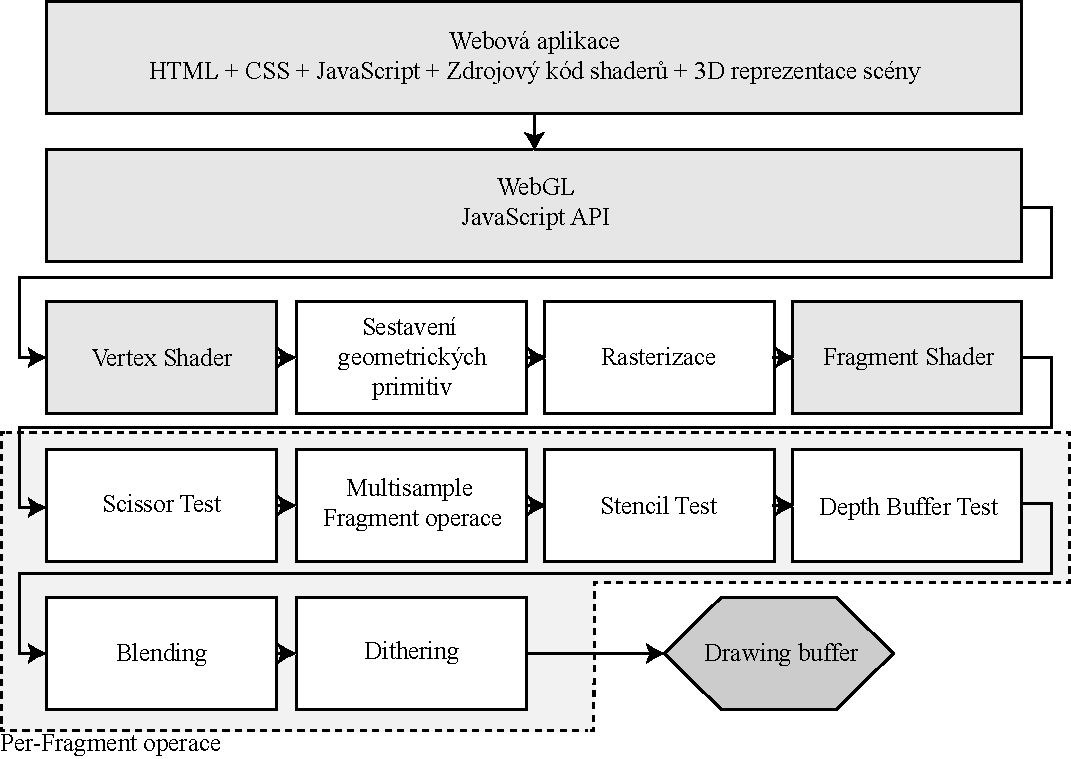
\includegraphics[width=0.8\textwidth]{gpuPipeline}
\caption{GPU pipeline}
\label{fig:gpuPipeline}
\end{figure}

K tomu, abychom získali realistickou 3D scénu nestačí pouze vykreslit objekty na určité pozice. Musíme také vzít v úvahu, jak budou objekty vypadat, pokud na ně bude dopadat světlo ze světelných zdrojů scény. Obecně se technice, která se používá ve spojitosti s působením světla na různé typy materiálů říká~\textit{shading}. Ve WebGL je shading rozdělen do dvou částí, jejichž chování je možné naprogramovat. \\ \\ Programovatelnými součástmi grafické pipeline jsou:
\begin{itemize}
\item Vertex Shader
\item Fragment Shader
\end{itemize}

\myparagraph{Vertex Shader}
První částí grafické pipeline, do které vstupují data předaná WebGL knihovně, je vertex shader. Jak již jeho název napovídá, provádí shading jednotlivých vertexů vykreslované scény. Než však samotný proces shadingu započne, je nutno vertexy transformovat a umístit tak objekt, jemuž vertexy náleží, na požadovanou pozici. Toho je docíleno pomocí transformačních matic, které jsou popsány v podkapitole~\ref{section:linearniAlgebra}. Vertex shader používá následující vstupy:
\begin{itemize}
\item Zdrojový kód vertex shaderu, který je zapsán v OpenGL ES Shading Language (GLSL ES).
\item Atributy, které definují data specifická každému vertexu. Typicky je to jeho pozice, normála a barva.
\item Tzv. \textit{uniform} proměnné, které jsou pro všechny vertexy objektu konstantní a lze je změnit až po dokončení operace vykreslování. Jedná se o transformační matice a dále pak například o pozice, na kterých se nachází světelné zdroje.
\end{itemize}

\begin{figure}[htb]
\centering
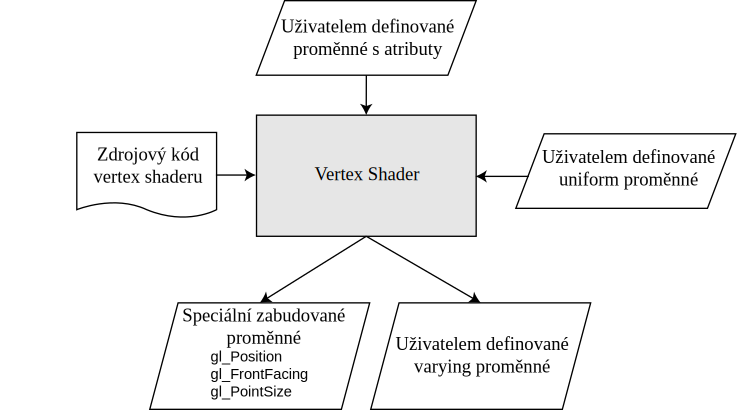
\includegraphics[width=0.8\textwidth]{vertexShader}
\caption{Vertex Shader}
\label{fig:vertexShader}
\end{figure}

Na diagramu~\ref{fig:vertexShader} jsou pak jestě znázorněny zabudované a uživatelky definované \textit{varying} proměnné. Využití varying proměnných je v delegaci informací z vertex shaderu do fragment shaderu. Jednou z nejdůležitějších speciálních zabudovaných proměnných je \texttt{gl\_Position}, která po práci vertex shaderu udává pozici, na které se vertex nachází. Popis vertex shaderu probíhá pomocí jazyka GLSL, který je svou syntaxí podobný programovacímu jazyku C. Příklad takového popisu je uveden ve zdrojovém kódu~\ref{code:vertexShader}

\begin{lstlisting}[caption=Ukázka zdrojového kódu GLSL pro vertex shader,label=code:vertexShader]
// Deklarace atributů vertexu
// Vektor pozice vertexu (XYZ)
attribute vec3 aVertexPos;
// Barva vertexu (RGBA)
attribute vec4 aVertexColor;

// Uniform proměnné
// Model-View Matice (4x4)
uniform mat4 uMVMatrix;
// Projekční matice (4x4)
uniform mat4 uPMatrix;

// Deklarace varying proměnné obsahující výstupní barvu vertexu, 
// která je vstupem pro fragment shader.
varying vec4 vColor;

void main() {
	// Transformace vertexu projekční a model-view maticí, kde
	// gl_Position udává jeho výslednou pozici ve scéně.
	gl_Position = UPMatrix * uMVMatrix * vec4(aVertexPos, 1.0);
	
	// Barva vertexu je poslána dále do fragment shaderu	.
	vColor = aVertexColor;
}
\end{lstlisting}
\pagebreak
\myparagraph{Sestavení primitiv}
V tomto kroku jsou sestaveny jednotlivé vertexy, které prošly skrze vertex shader, do geometrických primitiv, jakými jsou například trojúhelníky či hrany. Následně je potřeba rozhodnout o tom, zda je sestavený objekt v regionu, který je aktuálně viditelný na obrazovce. Tento region je označován jako \textit{frustrum} a je představován komolým jehlanem s obdélníkovou, či čtvercovou podstavou. Objekt který je uvnitř frustra je předán ke zpracování dalším částem grafické pipeline. Objekty, které jsou kompletně mimo frustrum, se odstraní, a ty, které jsou vně pouze částečně, budou oříznuty. Frustrum je znázorněno na diagramu~\ref{fig:frustrum}

\begin{figure}[htb]
\centering
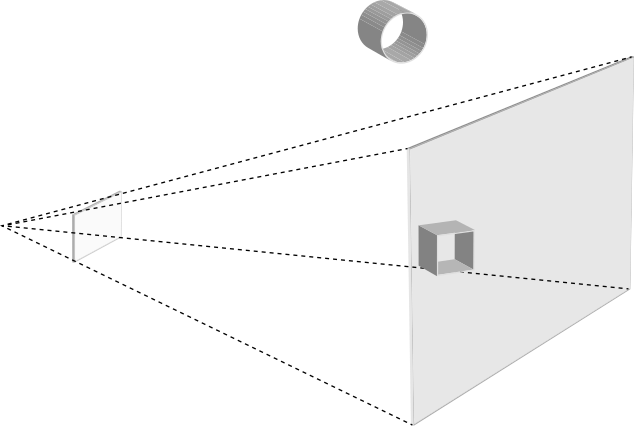
\includegraphics[width=0.8\textwidth]{frustrum}
\caption{Frustrum}
\label{fig:frustrum}
\end{figure}

\myparagraph{Rasterizace}
Dalším krokem je převod primitiv na fragmenty (diagram~\ref{fig:planeFragment}), pod kterými si můžeme představit jednotlivé pixely obrazovky. Fragmenty dále putují do fragment shaderu.

\begin{figure}[htb]
\centering
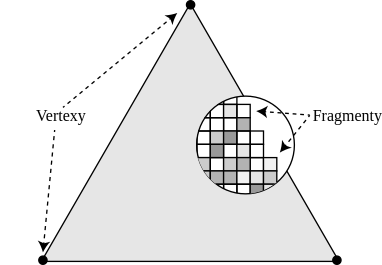
\includegraphics[width=0.8\textwidth]{planeFragment}
\caption{Fragmenty}
\label{fig:planeFragment}
\end{figure}

\myparagraph{Fragment shader}
Fragment shader je druhou programovatelnou součástí grafické pipeline. Jak již bylo zmíněno, fragment odpovídá pixelu, avšak ne všechny fragmenty se pixely stanou. Fragmenty totiž mohou být odstraněny v dalších částech pipeline. Fragment shader se svými vstupy a výstupy je znázorněn na diagramu~\ref{fig:fragmentShader}. Vstupem fragment shaderu jsou:
\begin{itemize}
\item Zdrojový kód fragment shaderu v jazyku OpenGL ES Shading Language.
\item Speciální zabudované proměnné, mezi něž patří například \texttt{gl\_PointCoord}.
\item Varying proměnné, které byli poslány skrze vertex shader.
\item Uniform proměnné, které obsahují konstanty společné všem fragmentům vykreslovaného objektu.
\item Samplery, což jsou speciální uniform proměnné určené pro texturování.
\end{itemize}

\begin{figure}[htb]
\centering
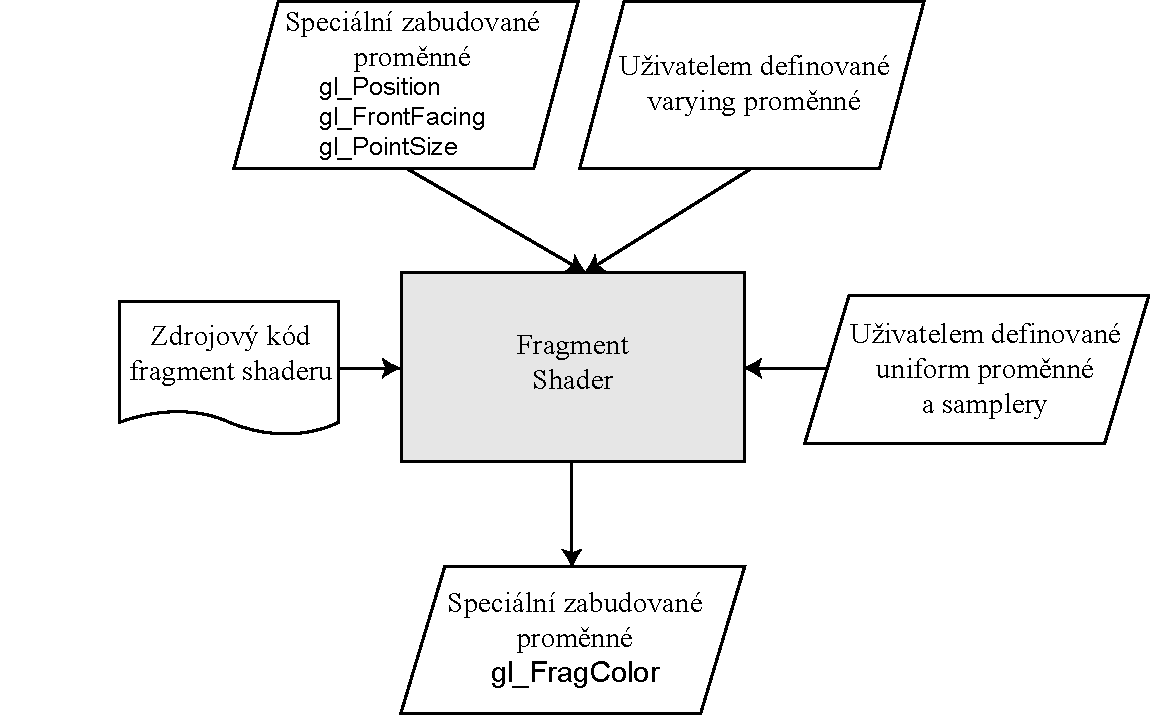
\includegraphics[width=0.8\textwidth]{fragmentShader}
\caption{Fragment Shader}
\label{fig:fragmentShader}
\end{figure}



Jak již bylo zmíněno dříve, varying proměnné slouží k posílání informací skrze vertex shader. Obecně však platí, že objekt má více fragmentů než vertexů. Obsah varying proměnných, který je zaslán skrze vertex shader, je lineárně interpolován pro každý fragment. 

Výsledek práce fragment shaderu je zapsán do zabudované proměnné \texttt{gl\_FragColor}, která následně obsahuje výslednou barvu daného fragmentu. Ve zdrojovém kódu~\ref{code:fragmentShader} je uveden příklad GLSL programu fragment shaderu, který pro každý fragment získá lineárně interpolovanou hodnotu s jeho barvou a uloží ji jako svůj výstup.

\label{code:fragmentShader}
\begin{lstlisting}[caption=Příklad jednoduchého GLSL programu fragment shaderu]
varying ver4 vColor;
void main(){
	gl_FragColor = vColor;
}
\end{lstlisting}

\myparagraph{Per-Fragment operace}
Každý fragment, který projde fragment shaderem, je postoupen do dalšího bloku pipeline, která se skládá z několika částí provádějící tzv. per-fragment operace. Každá z operací může ovlivnit výsledný pixel v drawing bufferu, avšak v implementaci je využito pouze blendingu a depth buffer testu. Zbylé části jsou uvedeny pro úplnost popisu pipeline.

\mysubparagraph{Scissor test}
Scissor test určuje, zda je zpracovávaný fragment uvnitř pravoúhlého rovnoběžníku, který je definován jedním bodem, výškou a šírkou. Fragmenty mimo tento rovnoběžník jsou zahozeny, ostatní pokračují dále v cestě grafickou pipeline.

\mysubparagraph{Multisample fragment operace}
Tato část pipeline modifikuje aplha kanál fragmentu, čímž je docíleno vyhlazení hran vykreslovaných objektů. Tato technika se obecně označuje jako \textit{anti-aliasing}.

\mysubparagraph{Stencil test}
Zde se fragment porovnává s nastavenou referenční hodnotou. Na základě výsledku porovnání je fragment opět zahozen, nebo postoupen dále.

\mysubparagraph{Depth buffer test}
Vzhledem k tomu, že se v téměř každé vykreslované scéně objekty překrývají, je nutné do color bufferu vykreslovat pouze ty objekty, které jsou viditelné. Tento test ve spolupráci s depth bufferem rozhoduje o tom, zda fragment vykreslovat, či nikoliv.

\mysubparagraph{Blending}
V dalším kroku označovaným jako blending jsou kombinovány barvy fragmentů, které jsou momentálně vykresleny do color bufferu na odpovídající pozici. Toho je v implementaci využito pro vykreslování průhledných objektů scény.

\mysubparagraph{Dithering}
Posledním krokem před vykreslením do color drawing bufferu je tzv. dithering. Vzhledem k tomu, že color buffer má omezený počet bitů k reprezentaci každé z barev, dithering tyto složí tak, že vytvoří iluzi toho, že máme k dispozici barev více.

%\subsection*{WebGL Frameworky}
%\label{subsection:webGLFrameworky}
%Specifikace neexistuje dlouhou dobu, avšak již dnes můžeme nalézt mnohé frameworky, které programování s WebGL značně usnadňují. Vzhledem k tomu, že použití WebGL frameworků nebylo při implementaci povoleno, má následující přehled pouze informativní charakter.

%Mezi nejznámější WebGL frameworky patří:
%\begin{itemize}
%\item C3DL
%\item Copperlicht
%\item GLGE
%\item SceneJS
%\item Three.js
%\item WebGLU
%\end{itemize}

%\subsection*{WebGL a bezpečnost}
%WebGL přistupuje přímo ke grafickému hardwaru, tudíž se mohou objevit situace, ve kterých je možné tuto skutečnost zneužít a vytvořit takový %WebGL dokument, který způsobí to, že grafická karta přestane reagovat na ostatní aplikace. Systémy Microsoft Windows tuto skutečnost detekují a %resetují grafickou kartu, avšak na systémech firmy Apple není tato detekce přítomna a takový dokument by potenciálně mohl zapříčinit pád %systému. U Linuxu záleží na verzi použitého ovladače grafické karty. Některé z nich blokaci detekují a některé nikoliv (například současný %ovladač grafických karet NVIDIA Nouveau). 

%\subsection*{Rychlost JavaScriptu v souvislosti s WebGL}
%Interprety JavaScriptu v prohlížečích se neustále vylepšují a dosahují tak vyšších rychlostí, avšak pro výpočetně složité operace je jeho %rychlost stále nízká. Pokud tedy chceme dosáhnout rychlého vykreslování, je potřeba přenechat co nejvíce práce grafickému hardwaru a jeho %shaderům. Na diagramu~\ref{webglPerformace} je uvedeno srovnání jednotlivých webových prohlížečů s  

%doplnit osvetlovaci modely a opacity



\chapter{Koncepce hry}
\label{chap:analysis}
Návrh implementované hry zakládá na analýze hry Berušky 2, která byla provedena metodou \textit{černé skříňky}\footnote{Na základě akcí uživatele byla zkoumána reakce hry s tím, že princip vnitřní implementace zůstal utajen.}. Hra je nejprve stručně představena a následně jsou uvedeny výsledky herní analýzy, na kterých zakládá implementace~\ref{chap:implementace}

\section{Berušky 2}
Berušky 2, neboli také Berušky 3D, jsou pokračováním logické hry vývojářského týmu Anakreon\footnote{\url{www.anakreon.cz}}, jehož členem je pan Ing. Martin Stránský, který byl konzultantem této bakalářské práce. Oproti své první, volně dostupné verzi, bylo toto pokračování od počátku vytvářeno jako komerční produkt. Hra byla od roku 2004 distribuována v České republice a některých dalších zemích společností Cinemax. V březnu roku 2011 byla část této hry uvolněna pod open-source licencí a je dále vyvíjena panem Stránským. První verze hry Berušky je svou koncepcí velmi podobná hře Sokoban~\footnote{\url{https://en.wikipedia.org/wiki/Sokoban}}. Druhá verze hry se svou koncepcí příliš od prvního dílu neodlišuje, avšak do hry přibyly nové herní prvky, a co je hlavní, hra je kompletně ve 3D. Každá úroveň této hry je logickou hříčkou, která ke svému řešení vyžaduje volbu správného plánu a dávku trpělivosti. Každá z berušek má schopnost před sebou tlačit bedny a používat herní předměty, čímž vytváří cestu k cíli, avšak pro jeho dosažení je často důležité, aby spolu berušky vzájemně spolupracovali.

Původní hra distribuovaná firmou Cinemax obsahuje celkově 160 herních úrovní včetně 20 tutoriálů a 45 jednodušších úrovní, které jsou určeny pro mladší hráče a trénink. Hlavní součástí hry je pak \textit{Beruščí cesta}, která obsahuje celkem 95 úrovní rozdělených do 9 epizod odehrávajících se v různých prostředích. Open-source verze hry pak obsahuje tutoriály, některé tréninkové úrovně a 3 z úrovní Beruščí cesty.

\section{Herní pole}
Herní pole je ve tvaru krychle či kvádru a je rozděleno na jednotlivé pozice, ve kterých jsou umístěny jeho prvky (diagram~\ref{fig:gameField}). Nikdy nemůže dojít k situaci, že by se herní prvek včetně berušek vyskytl mimo herní pole. Po prvcích jako jsou bedny, či zeď je možné se volně pohybovat, avšak beruška nikdy nemůže z vyšší herní pozice seskočit dolů.

\begin{figure}[htb]
\centering
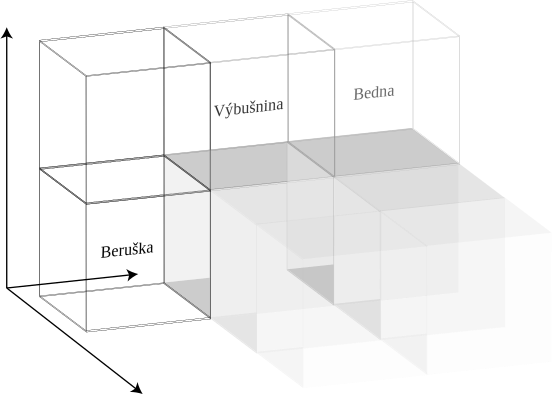
\includegraphics[width=0.8\textwidth]{gameField}
\caption{Herní pole a jeho prvky}
\label{fig:gameField}
\end{figure}

\section{Prvky herního pole}
Jak již bylo uvedeno, v rámci herního pole jsou umístěny prvky, jejichž rozmístění představuje samotnou logickou hříčku, kterou hráč řeší. Prvky se od sebe liší nejen funkčností a vzhledem, ale také tím, že některé z nich jsou umístěny staticky (hráč s nimi nemůže pohnout) a některé z nich jsou dynamické (bedny, výbušniny, \ldots). Následuje přehled prvků herního pole a jejich stručný popis.

\myparagraph{Beruška}  %\item[Beruška] \hfill \\
V každé herní úrovni se vyskytuje 1-5 berušek, které jsou ovládány hráčem. Berušky mohou pohybovat bednami, či výbušninami za účelem vytvoření cesty k východu. Každá z nich má inventář, který obsahuje předměty, které beruška při svém pohybu herním polem získala. 
\myparagraph{Zeď}  %\item[Zeď] \hfill \\
Zeď je jedním ze statických prvků, který má ve svém herním poli stálou pozici a nelze ho nijak odstranit. Beruška se po zdech může volně pohybovat.
\myparagraph{Východ}  %\item[Východ] \hfill \\
Cílem je dostat všechny berušky do východu. Stejně jako zeď je i východ umístěn stále na stejné pozici.
\myparagraph{Bedna} % \item[Bedna] \hfill \\
Bedna je základním herním prvkem, který beruška tlačí před sebou a vytváří tak cestu k cíli. Počet přesouvaných beden je závislý na aktuální síle berušky (podkapitola~\ref{section:weight}) a je možné je odstranit pomocí výbušniny. Bedny lze také tlačit po šikmé podlaze a dostat je tak do vyšší, či nižší úrovně herního pole. Podle váhy pak rozlišujeme bedny na lehké a těžké.
\myparagraph{Výbušnina}%\item[Výbušnina] \hfill \\
Výbušnina je prvkem, který se po většinu času chová jako obyčejná bedna, avšak pokud je \uv{natlačena} na některou z beden, pak dojde k výbuchu. Bližší popis toho, jak výbuchy probíhají, je v podkapitole~\ref{section:explosive}.
\myparagraph{Kámen}%\item[Kámen] \hfill \\
Kámen představuje překážku, kterou nelze posunout, avšak je možné ho odstranit pomocí krompáče, který může beruška nalézt při průchodu herním polem.
\myparagraph{Voda}%\item[Voda] \hfill \\
Voda je pro berušku další překážkou. Pokud je v dané herní úrovni voda, pak musí beruška s největší pravděpodobností pod vodní hladinu, kde získá potřebný předmět. Někdy se dokonce pod vodní hladinou nachází i východ z úrovně, avšak v každém případě beruška potřebuje šnorchl, aby se mohla potopit. Ten může stejně jako krompáč získat při průchodu herním polem. 
\myparagraph{Krompáč}%\item[Krompáč] \hfill \\
Krompáč je předmět, který se používá pro odstranění kamene. Maximální počet krompáčů, který může mít jedna beruška v inventáři, je 4. Po použití je krompáč odstraněn z inventáře.
\myparagraph{Šnorchl}%\item[Šnorchl] \hfill \\
Beruška ho potřebuje, aby se mohla potopit pod vodní hladinu. Pokud beruška tento předmět nemá ve svém inventáři, pak je zamezeno jakémukoliv hernímu kroku, kterým by se beruška mohla pod hladinu dostat.
\myparagraph{Závaží}%\item[Závaží] \hfill \\
Závaží dvojnásobně zvyšuje váhu berušky. Toho se využívá v situacích, kdy potřebujeme, aby se pod beruškou propadla podlaha. 
\myparagraph{Hormonální vitamín}%\item[Hormonální vitamín] \hfill \\
Pokud beruška získá hormonální vitamín, pak získá dvojnásobnou sílu, což ji následně umožňuje před sebou tlačit více beden.
\myparagraph{Bortící se podlaha}%\item[Bortící se podlaha] \hfill \\
Občas se hře vyskytuje i podlaha, která se propadá pod vahou, která je nad ní naskladněna. Bližší informace o vahách herních prvků jsou uvedeny v podkapitole~\ref{section:weight}.
\myparagraph{Šikmina}%\item[Šikmina] \hfill \\
Šikmina je posledním z herních prvků. Umožňuje berušce sestoupit, či vystoupit z/do vyšší úrovně herního pole. Zároveň je možné po šikmině pohybovat bednami a výbušninami.

\section{Váhy herních prvků a síla berušky}
\label{section:weight}
Ve hře hraje velkou roli váha, která je přiřazena každému z prvků. Ta rozhoduje o tom, zda je beruška schopná posunout prvky, které se před ní nacházejí, a také o tom, zda se pod nimi nepropadne podlaha. Základní síla berušky, resp. to, kolik váhy před sebou může tlačit, jsou 2 váhové jednotky. S hormonálním vitamínem ve svém inventáři je pak síla berušky navýšena na 4 váhové jednotky. Bortící se podlaha nad sebou udrží pouze 1 váhovou jednotku a může na ni tedy být natlačena lehká bedna, nebo si na ni může stoupnout beruška, která ve svém inventáři nemá závaží. Při překročení váhy se podlaha propadne a objekty, které na ní byly naskládány, změní svou vertikální pozici tak, aby pod sebou měly podklad. Zajímají nás pouze váhy prvků, se kterými je možné ve hře pohybovat. Přehled dynamických prvků a jejich vah je uveden v tabulce~\ref{table:weights}.

\begin{table}
\label{table:weights}
\begin{center}
    \begin{tabular}{ | l | l |}
    \hline
    \textbf{Prvek} & \textbf{Váha} \\ \hline
    Beruška & 1 \\ \hline
    Lehká bedna & 1 \\ \hline
    Těžká bedna & 2 \\ \hline
	Výbušná bedna & 2 \\ \hline
    \end{tabular}

\end{center}
\caption{Váhy dynamických prvků}
\end{table}

\section{Posuvy beden}
Bedny jsou ve hře na různých pozicích a často jsou umístěny za sebou. O tom, zda beruška může provést posuv jedné či více beden rozhoduje více faktorů. 

\begin{itemize}
\item Aktuální beruščina síla. 
\item Obsah pozice za poslední posouvanou bednou.
\item Součet vah posouvaných beden.
\end{itemize} 

Pokud uvažujeme posuv jedné jediné bedny, pak je situace jednoduchá. Zjistí se obsah pozice, kam má být bedna posunuta, a pokud je tato pozice prázdná, pak se posun provede. Při posuvu více beden najednou je potřeba spočítat souhrnnou váhu posouvaných beden a určit obsah pozice, na kterou bude posunuta od berušky nejvzdálenější z nich. Jakmile má beruška dostatečnou sílu k posunu a konečná pozice je prázdná, pak je posun proveden. V opačném případě zůstává beruška i bedny na svém původním místě.

Je také důležité zdůraznit, že bedny mohou být posunuty do míst, kde pod sebou nemají žádný podklad. V takových situacích je pozice těchto beden upravena tak, aby pod sebou měly nějaký prvek.

\section{Výbušné bedny}
\label{section:explosive}
Výbušnými bednami lze ve většině situací normálně pohybovat. Změna nastává v případě, kdy je před výbušninou bedna obyčejná. V takové situaci je na ni výbušná bedna \uv{nasunuta} a dochází k výbuchu. Při výbuchu jsou obě bedny odstraněny a je upravena vertikální pozice prvků, které se nad nimi před výbuchem nacházely. Posouvanými prvky mohou být další výbušné bedny a ty při posunu vždy odstraní obyčejné, které se nacházejí pod nimi. 

Na diagramu~\ref{fig:bangDiagram} je ukázka komplexního výbuchu. Váha beden zde značně přesahuje beruščinu sílu, avšak za výbušnou bednou do které beruška tlačí je bedna obyčejná. Dojde tedy k výbuchu, odstranění beden a \uv{pádu} těch, které se nad nimi nacházely. Při pádu jsou odstraňovány bedny, které nad sebou mají výbušninu a zbude pouze jediná. Ta se nakonec bude nacházet přímo před beruškou, která zůstává na své původní pozici.

\begin{figure}[htb]
\centering
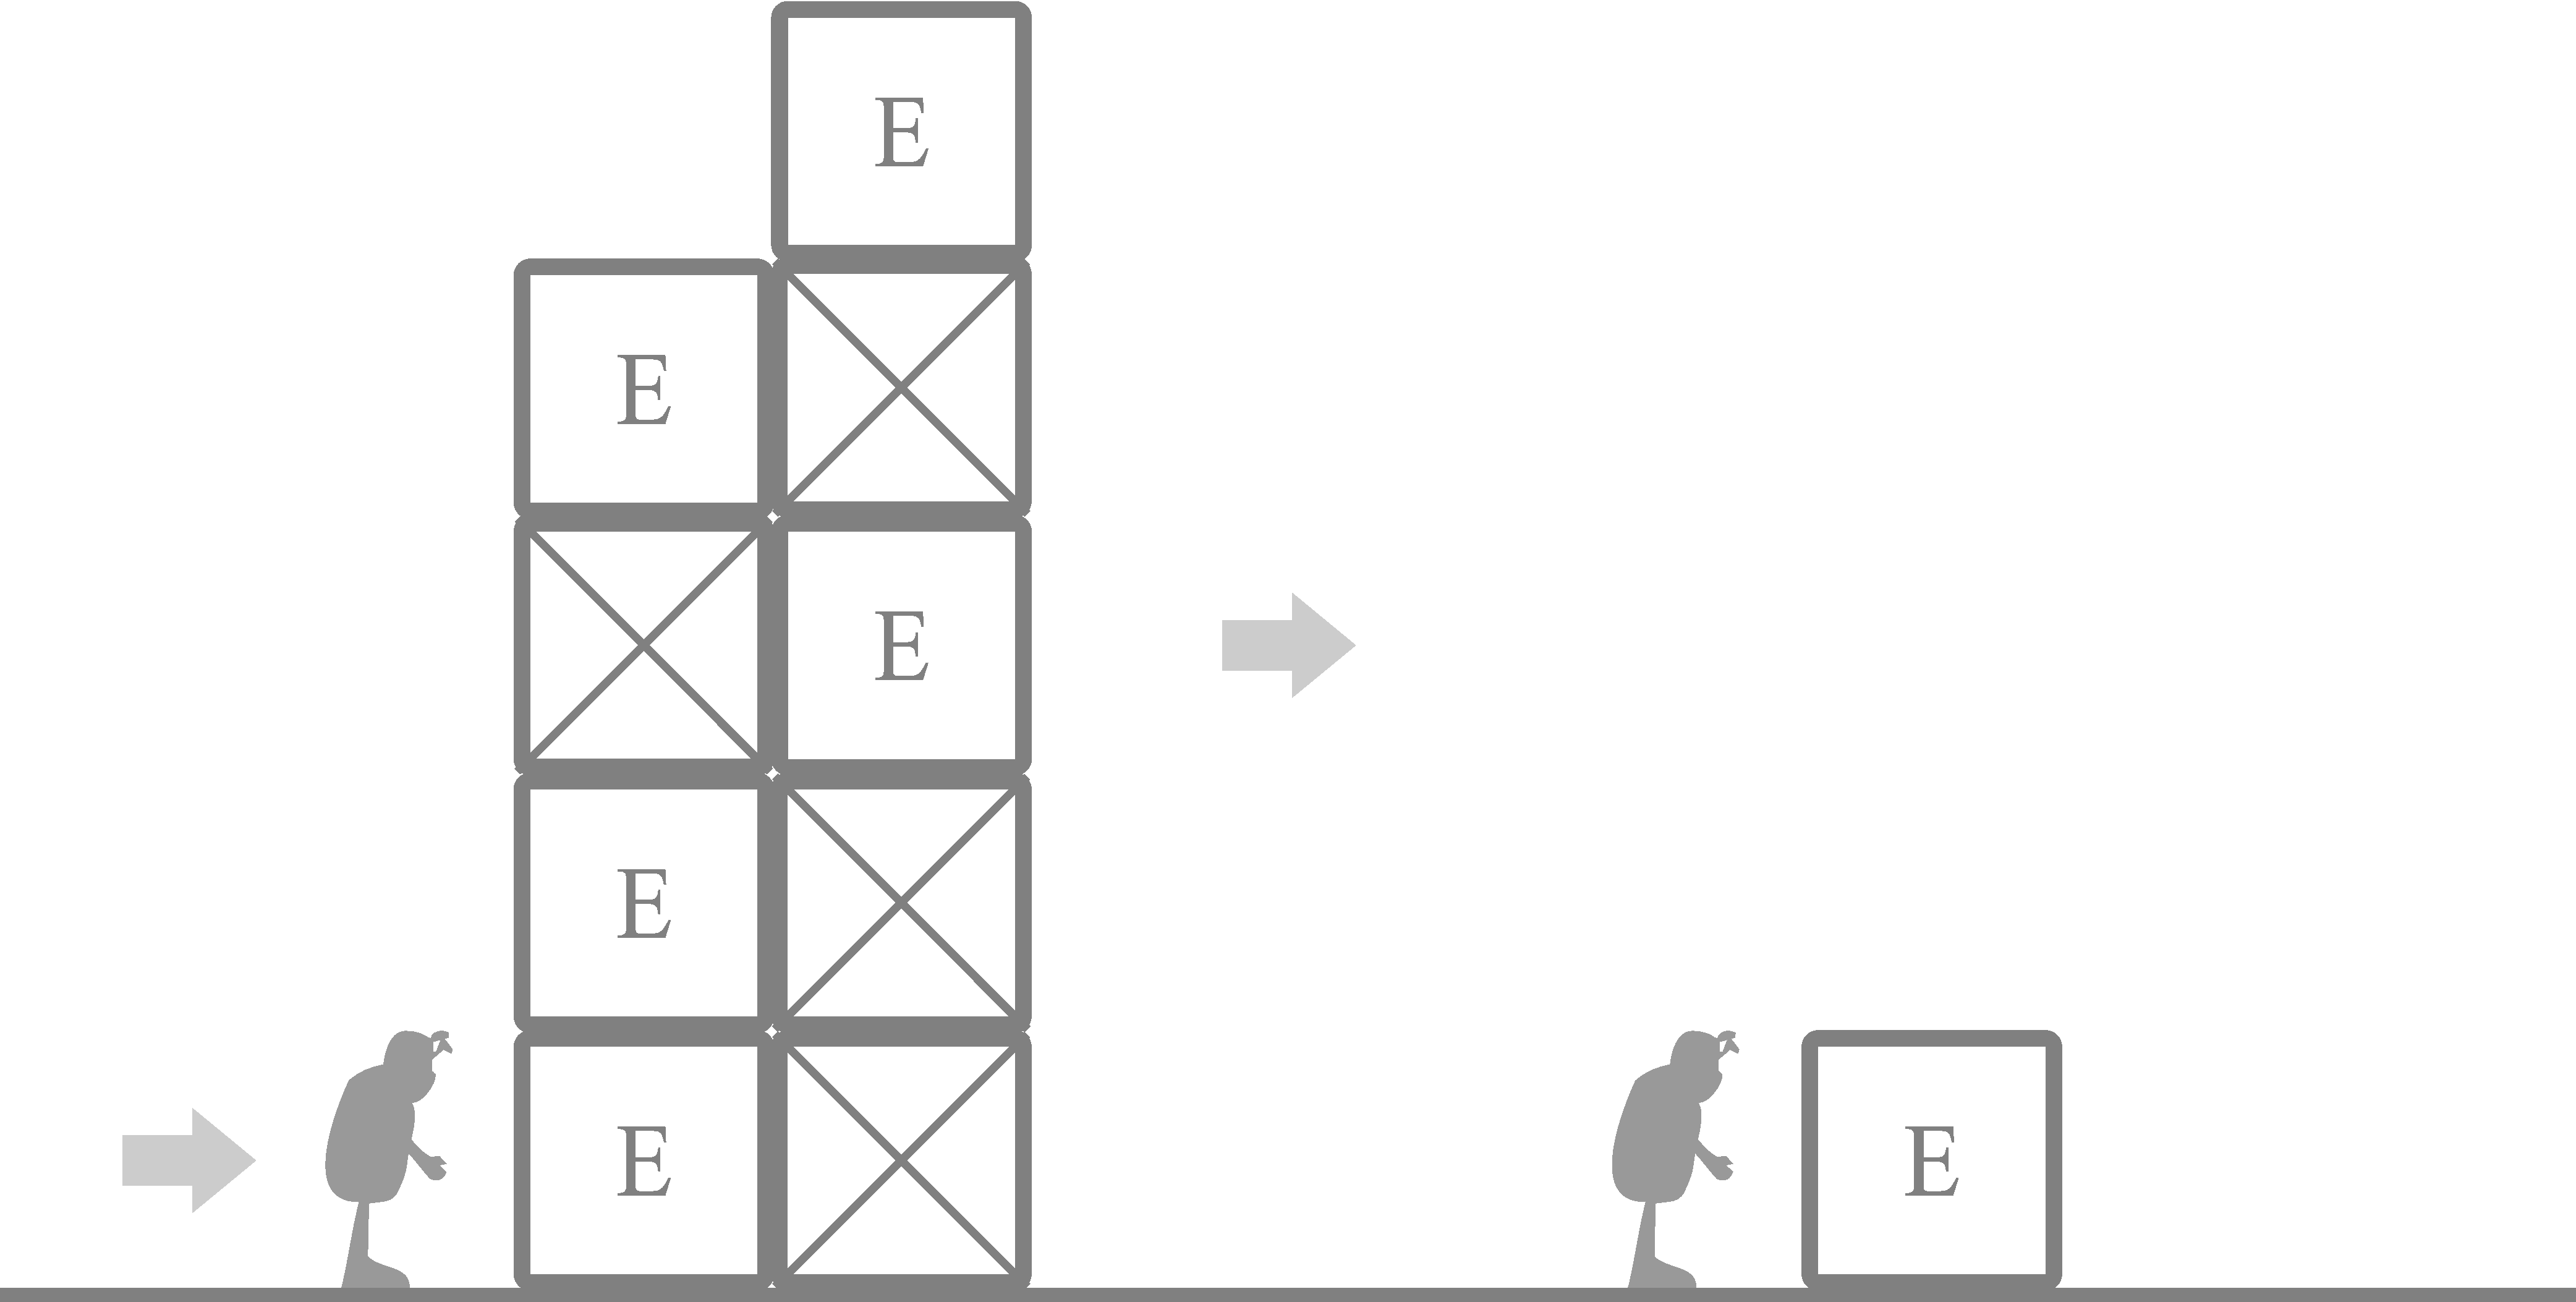
\includegraphics[width=0.8\textwidth]{bangDiagram}
\caption{Ukázka komplexního výbuchu}
\label{fig:bangDiagram}
\end{figure}

\section{Ovládání}
Berušky jsou vybírány pomocí kláves \keystroke{1} až \keystroke{5} a je s nimi pohybováno pomocí šipek. Důležité je ovládání kamery, která rotuje kolem momentálně vybrané berušky pohybem myši na okraj herní obrazovky. Pokud nemá uživatel přímou viditelnost na vybranou berušku, pak může objekty, které se mezi ním a beruškou nacházejí, nechat zprůhlednit pomocí mezerníku. Tlačítkem \Enter je pak pozice kamery přesunuta nad herní pole. 

\section{Vykreslování}
\label{section:navrhVykreslovani}
Informace týkající se technologie vykreslování jsou uvedeny v následujícím odstavci. Jejich přítomnost nechť čtenář bere pouze jako zajímavost, jelikož implementace hry, která je součástí této práce, probíhala nezávisle na hře původní. Jediným převzatým materiálem byla, jak se čtenář dále dozví, data pro zobrazení herní úrovně. 

V původní hře je celá scéna organizována jako strom hierarchických OBB obálek. Při vykreslování je pak strom procházen a je zjišťována viditelnost jednotlivých obálek. Osvětlovací model je kombinovaný z per-vertex shadingu a lightmap. Hra obsahuje také mnohé animace, které jsou u berušek realizovány jako objektové a pro zbytek objektů scény jako mesh animace. Aktuálně vyvíjená open-source varianta hry obsahuje také například zrcadlový rendering, kreslení odlesků, halo efekty, anisotropické filtrování textur, bump-mapping, komprimované textury a mip-mapping. Informace o uvedených technologiích vykreslování zde nebudou z důvodu omezeného rozsahu této práce uvedeny.

\section{Návrh webu}
Implementace této části nebyla přímou součástí této práce, a proto jejímu návrhu nebude věnován velký prostor. Návrh webu je možné vidět na diagramu~\ref{fig:web}. Web je rozdělen na 3~části a jejich popis se nachází v následujících odstavcích.


\subsection*{Menu}
Pomocí menu se volí kontexty obrazovky (viz. dále).
\subsection*{Obrazovka} Obrazovka je primárně určena k zobrazení aktuálně načtené herní úrovně. Pro ucelenost webu je však obrazovka využita i k zobrazení dalších informací a lze tedy rozpoznávat její jednotlivé kontexty. Těmi jsou:
	\begin{itemize}
	\item Hra

\item Informace o hře
\item Návod na hraní hry
\item Popis ovládání hry
	\end{itemize}
Při volbě herního kontextu se v rámci obrazovky zobrazí samotný element \texttt{<canvas>}, do kterého je vykreslována zvolená herní úroveň. V levém dolním rohu je zobrazen inventář aktuálně vybrané berušky a v rohu pravém je možné ovládat přehrávání herní hudby. Reakce na události vytvářené hráčem jsou zpracovány a o některých z nich je zobrazena notifikace, která tak dává hráči zpětnou vazbu. 
\subsection*{Výběr herních úrovní}
Tato část umožňuje uživateli vybrat z dostupných herních úrovní, které jsou následně vykreslovány do herního kontextu obrazovky. Mezi jednotlivými bloky pro výběr úrovně lze přecházet poklikem na šipky. Při jednom pokliku jsou úrovně posunuty o jeden blok a při pokliku dvojitém pak o bloky 4. Výběr by neměl obtěžovat hráče v okamžiku, kdy není potřeba. Proto je možné ho otevřít/skrýt pomocí tlačítka, které je umístěno ve spodní části obrazovky.



\chapter{Implementace}
\label{chap:implementace}
V kapitole~\ref{chap:analysis} byla analyzov�na hra Beru�ky 2, kter� se stala vzorem pro hru implementovanou v r�mci t�to pr�ce. Zp�sob, jak�m je hra implementov�na, je uveden na diagramu~\ref{fig:gameDiagram}. V n�sleduj�c� podkapitol�ch budou pops�ny jeho jednotliv� ��sti a t�m i objasn�na hern� architektura.

TODO...jak byla testovana funkcnost

\begin{figure}[htb]
\centering
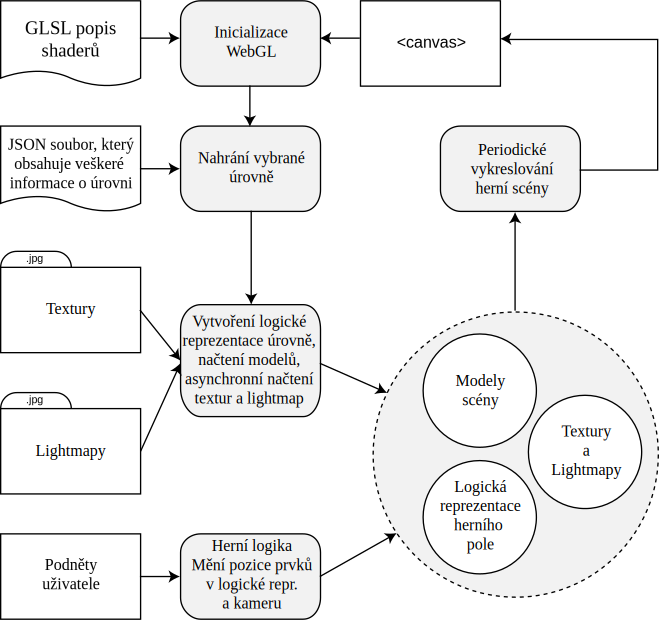
\includegraphics[width=0.8\textwidth]{gameDiagram}
\caption{Architektura hry Beru�ky 2 WebGL}
\label{fig:gameDiagram}
\end{figure}

\section{Inicializace}
Inicializace elementu \texttt{<canvas>} je prvn�m krokem, kter� je pot�eba vykonat. T�m, �e z�sk�me referenci na jeho \texttt{webgl} kontext, m��eme p�ej�t k dal��mu kroku, kter� nastav� vertex a fragment shadery. Popis funk�nosti shader� je proveden pomoc� jazyka GLSL, jeho� uk�zky byly uvedeny u popisu grafick� pipeline (\ref{subsection:pipeline}). Zdrojov� k�dy jsou obsa�eny v HTML dokumentu uvnit� t�chto elemtent�:
\begin{itemize}
\item Vertex Shader \\ \texttt{\textless script id="per-fragment-lighting-vs"\ type="x-shader/x-vertex"\textgreater}
\item Fragment Shader \\ \texttt{\textless script id="per-fragment-lighting-fs"\ type="x-shader/x-fragment"\textgreater}
\end{itemize}

V implementaci je hra inicializov�na pomoc� funkce \texttt{webGLStart()}, kter� mimo jin� nastavuje zp�sob zpracov�n� ud�lost� vytv��en�ch u�ivatelem.

\section{Nahr�n� vybran� �rovn�}
Po inicializaci je p�istoupeno k nahr�n� �rovn� vybran� hr��em. Ka�d� z �rovn� je p�edstavov�na samostatn�m JSON souborem, kter� je asynchronn� nahr�n (\ref{subsection:AJAX}) ze serveru.

\subsection*{JSON soubor}
\label{subsection:navrhJSON}
Tento soubor obsahuje kompletn� informace, kter� jsou pot�ebn� pro zobrazen� dan� hern� �rovn�. Jedn� se tak o hlavn� sou��st cel� hry, bez kter� by nemohla fungovat. Soubor vznik� exportem pot�ebn�ch informac� z p�vodn� hry a jeho hlavn� sou��sti jsou pops�ny v n�sleduj�c�ch odstavc�ch.

\myparagraph{Informace o materi�lech}
Materi�ly jsou pou�ity k otexturov�n� model�. Rozd�l mezi materi�lem a texturou je takov�, �e materi�l se obecn� m��e skl�dat z v�ce textur, kter� se pak vz�jemn� prol�naj�. Lze tak m�t nap��klad materi�l, kter� vznikne slo�en�m z textur zdi a mechu. V�hoda je v tom, �e slo�it�j�� textury lze slo�it z jednodu���ch a nen� tedy pot�eba uchov�vat nadbyte�n� data. Ka�d� z materi�l� m� v souboru jm�na textur, ze kter�ch se skl�d�, a tak� sv� unik�tn� jm�no, pomoc� n�ho� se n�sledn� objekty sc�ny na tento materi�l odkazuj�. Uk�zka popisu materi�lu je uvedena ve zdrojov�m k�du~\ref{code:jsonMaterial}.

\begin{lstlisting}[caption=Objekt \texttt{material} vstupn�ho souboru JSON,label=code:jsonMaterial]
{
  "type" : "material",
  "name" : "256_p-d1-256",
  "transparent" : "0",
  "z_buffer_mask" : "1",
  "z_buffer_test" : "1",
  "backface_culling" : "1",
  "diffuse_color" : "1",
  "specular_color" : "0",
  "textures" : [ "s1_0013.jpg" ]
}
\end{lstlisting}

\myparagraph{Ob�lky objekt� hern� sc�ny}
M�lokter� ze slo�it�j��ch objekt� je slo�en pouze z jednoho modelu. Ve chv�li, kdy celkov� model objektu rozd�l�me na ��sti, je mo�n� tyto ��sti samostatn� transformovat �i m�nit materi�l, kter� pou��vaj�. Av�ak v okam�ik, kdy chceme n�jak�m zp�sobem transformovat cel� objekt, je vhodn� m�t v�echny modely objektu v jak�si ob�lce. Tato ob�lka m� v souboru sv� identifika�n� ��slo, kter� slou�� k identifikaci v�ech jej�ch model�. Identifika�n� ��slo je pot�ebn� pouze tehdy, pokud pot�ebujeme s ob�lkou transformace prov�d�t a je tedy vyu�ito pouze u dynamick�ch objekt� hern� plochy.

\mysubparagraph{Modely}
Modely jsou v souboru reprezentov�ny strukturami, kter� obsahuj� informace o poloze model� v r�mci sc�ny, o jejich barv� �i nap��klad o materi�lech, kter� jsou jim p�i�azeny. N�kter� z model� maj� tak� dal�� textury s p�edpo��tan�mi st�ny pro realisti�t�j�� zobrazen� sc�ny - lightmapy. 

Ve zdrojov�m k�du~\ref{code:jsonContainer} je uveden zjednodu�en� popis ob�lky, kter� obsahuje 1 model. Identifika�n� ��slo \texttt{2} znamen�, �e se jedn� o dynamick� prvek sc�ny (pokud by se jednalo o statick� prvek, pak by ��slo bylo \texttt{-1}). Pomoc� polo�ky \texttt{material} se model v tomto p��pad� odkazuje na materi�l, kter� byl pops�n ve zdrojov�m k�du~\ref{code:jsonMaterial}. Trojice prvk� v poli \texttt{vertexPositions} v�dy ud�v� pozici vertexu ve sc�n�. O tom, kter� vertexy n�le�� geometrick�m primitiv�m, ze kter�ch je model slo�en, rozhoduje pole \texttt{indices}. Zbyl� polo�ky pak obsahuj� informace pot�ebn� pro spr�vn� namapov�n� materi�l� a lightmap.

\begin{lstlisting}[caption=Objekt \texttt{geometry\_container} vstupn�ho souboru JSON,label=code:jsonContainer]
{
  "type" : "geometry_container",
  "name" : "exit.b2m",
  "container_id" : "2",
  "poly_id" : "17",
  "prvek" : "1",
  "geometry_objects" : [
   {
    "name" : "exit.b2m",
    "material" : "256_p-d1-256",
    "vertexPositions" : [-27.586000,2.008000,-34.421001,-27.586000,0.008000,-36.421001,
         47.704437,85.772964,6.669896,130.704437,85.772964,-3.330104],
    "vertexNormals" : [-1.000000,0.000000,0.000000,-1.000000,0.000000,0.000000],
    "vertexTextureCoords0" : [1.000000,1.000000,0.000000,0.000000,1.000000,0.000000],
    "vertexTextureCoords1" : [1.000000,1.000000,0.000000,0.000000,1.000000,0.000000],
    "vertexTextureCoordsLight" : [0.140625,0.328125,0.171875,0.328125,0.156250,0.359375],
    "indices" : [0,1,2,3,0,5]
   }
  ]
}
\end{lstlisting}

\myparagraph{Logick� reprezentace hern�ho pole}
Ob�lky model� neobsahuj� ��dnou informaci o tom, jak� typ objektu ve sc�n� p�edstavuj�. Z tohoto d�vodu je nutn� rozli�it to, co je vykreslov�no na obrazovku, a s ��m pracuje logika hry. Jak ji� bylo uvedeno v kapitole~\ref{chap:analysis}, hern� pole je krychlov� �i kv�drov� a je slo�eno z jednotliv�ch pozic, na kter�ch se mohou nach�zet hern� prvky. Je to pr�v� logick� reprezentace hern�ho pole, kter� obsahuje informace o tom, kter� prvek se na kter� pozici nach�z�. Ka�d� prvek logick� reprezentace hern�ho pole m� op�t sv� identifika�n� ��slo, pomoc� kter�ho se odkazuje na ob�lku modelu, kter� ur�uje jeho vzhled.  

Ve zdrojov�m k�du~\ref{code:jsonLogic} je uveden popis hern�ho pole o velikosti $6\times6$ a v��ce $8$. Polo�ka \texttt{level\_start} ud�v� pozici, na kterou maj� b�t p�esunuty dynamick� objekty, kter� jsou norm�ln� um�st�ny v po��tku sou�adn�ho syst�mu sc�ny. Hern� pole zde obsahuje pouze jeden prvek, jeho� typ je ur�en polo�kami \texttt{class} a \texttt{subclass} (identifik�tory v�ech prvk� jsou uvedeny v tabulce~\ref{table:itemClass}). Logick� prvek se v tomto p��kladu pomoc� \texttt{container\_id} odkazuje na model, kter� byl pops�n ve zdrojov�m k�du~\ref{code:jsonContainer}. 

\label{code:jsonLogic}
\begin{lstlisting}
{
  "type" : "level_logic",
  "logic_level_size" : [ 6, 8, 6],
  "level_start" : [ 21.586000, -1.992000, -46.421001],
  "item_size" : "2",
  "level_items_num" : "1",
  "level_items" : [{
    "name" : "Exit - teleport - 1",
    "guid" : "4000",
    "class" : "4",
    "subclass" : "-1",
    "position" : [ 0, 5, 1 ],
    "rotation" : "0",
    "container_id" : "2"
  }]
}
\end{lstlisting}

\begin{table}
\label{table:itemClass}
\begin{center}
\begin{tabular}{ | l | l | l |}
\hline
\textbf{Prvek} & \textbf{itemClass} & \textbf{itemSubclass} \\ \hline
Beru�ka & 1 & 0 \\ \hline
Ze� & 2 & 0 \\ \hline
V�chod & 4 & 0 \\ \hline
Bedna & 5 & 0 \\ \hline
T�k� bedna & 5 & 0 \\ \hline
Lehk� bedna & 5 & 1 \\ \hline
V�bu�nina & 6 & 0 \\ \hline
K�men & 7 & 0 \\ \hline
Voda & 12 & 0 \\ \hline
�norchl & 13 & 0 \\ \hline
Hormon�ln� vitam�n & 13 & 5 \\ \hline
Z�va�� & 13 & 7 \\ \hline
Kromp�� & 13 & 8 \\ \hline
Bort�c� se podlaha & 15 & 0 \\ \hline
�ikmina & 19 & 0 \\ \hline
\end{tabular}
\end{center}
\caption{T��dy a podt��dy prvk� hern�ho pole}
\end{table}

Jak si mohl pozorn� �ten�� v�imnout, ��sla, kter� ozna�uj� typ prvku, nejdou sekven�n� za sebou. Je to zp�sobeno t�m, �e p�vodn� n�vrh hry Beru�ky 2 (desktopov� verze) obsahoval v�ce typ� hern�ch prvk�, ne� jich bylo nakonec implementov�no. 

\section{Vytvo�en� vnit�n� reprezentace hern� �rovn�}
Ka�d� struktu�e vyskytuj�c� se v JSON souboru (pops�no v~\ref{subsection:navrhJSON}) p��slu�� odpov�daj�c� objekty a po jeho asynchronn�m na�ten� je soubor zpracov�n pomoc� funkce \texttt{handleLoadedJSON}. Ta tento soubor sekven�n� proch�z�, rozpozn�v� jeho jednotliv� struktury a n�sledn� pomoc� JavaScriptov�ch konstruktor� vytv��� odpov�daj�c� objekty, se kter�mi hra pracuje. V n�sleduj�c�ch odstavc�ch je uveden p�ehled t�chto konstruktor� s jejich stru�n�m popisem.

\myparagraph{\texttt{Material}}
P�i vytv��en� objektu t�mto konstruktorem jsou ze serveru asynchronn� (\ref{subsection:AJAX}) nahr�ny textury, kter� materi�l vyu��v�. Z t�ch jsou n�sledn� vytvo�eny texturovac� buffery, kter� jsou nahr�ny do grafick� pam�ti. T�m, �e jsou do t�to pam�ti um�st�ny, je pak dosa�eno rychlej��ho vykreslov�n� cel� hern� sc�ny. Buffery jsou nastaveny tak, �e pokud je textura oproti sv� p�vodn� velikosti zv�t�ov�na (upscaling), pak se pou�ije line�rn� filtr, kter� na z�klad� okoln�ch pixel� dopo��t� line�rn� interpolac� barvu pixelu mezi nimi. Pro textury, kter� jsou naopak zmen�ov�ny je vygenerov�na mipmapa, ze kter� se pak vyb�r� nejvhodn�j�� verze textury. V�echny materi�ly jsou uchov�v�ny v asociativn�m poli \texttt{materials}, kde jednotliv� kl��e tohoto pole jsou samotn� n�zvy materi�l�. 

Ve zdrojov�m k�du~\ref{code:loadingMaterial} je uveden p��klad nahr�n� texturovac�ho bufferu vznikl�ho na�ten�m prvn� textury materi�lu uveden�ho ve zdrojov�m k�du~\ref{code:jsonMaterial} do grafick� pam�ti.

\begin{lstlisting}[caption=P��klad nahr�n� textury do grafick� pam�ti,label=code:loadingMaterial]
// ...	
// Textura je zrcadlov� obr�cena kolem osy Y
// WebGL pou��v� jin� sou�adn� syst�m
gl.pixelStorei(gl.UNPACK_FLIP_Y_WEBGL, true);
// Nastaven� aktu�ln� zpracov�van�ho bufferu textury
gl.bindTexture(gl.TEXTURE_2D, materials["256_p-d1-256"].buffers[0]); 
// Nahr�n� textury do grafick� pam�ti
gl.texImage2D(gl.TEXTURE_2D, 0, gl.RGBA, gl.RGBA, gl.UNSIGNED_BYTE, 
              that.textures[temp].image);
// Nastaven� filtru, kter�m bude textura zv�t�ov�na
gl.texParameteri(gl.TEXTURE_2D, gl.TEXTURE_MAG_FILTER, gl.LINEAR);
// Nastaven� filtru, kter�m bude textura zmen�ov�na
gl.texParameteri(gl.TEXTURE_2D, gl.TEXTURE_MIN_FILTER, 
                 gl.LINEAR_MIPMAP_NEAREST);
// Vygenerov�n� mipmapy
gl.generateMipmap(gl.TEXTURE_2D);
// ...
\end{lstlisting}

\myparagraph{\texttt{Lightmap}}
Objekt vytvo�en� t�mto konstruktorem je a� na p�r detail� stejn� jako objekt konstruktoru \texttt{Material}. Lightmapy jsou takt� na��t�ny asynchronn� a ukl�d�ny do pam�ti grafick� karty, av�ak vzhledem k tomu, �e se z p�vodn� hry nepoda�ilo v�echny lightmapy vyexportovat, je jejich pou�it� vypnuto.

\myparagraph{\texttt{GeometryContainer}}
\label{paragraph:ob�lky}
Tento konstruktor vytv��� ob�lku jednotliv�ch model� hern� sc�ny. Podle toho, zda ob�lka obsahuje identifika�n� ��slo, rozli�ujeme mezi ob�lkami dynamick�ch a statick�ch objekt� sc�ny a um�s�ujeme je do odpov�daj�c�ch pol�. Pro dynamick� ob�lky je to asociativn� pole \texttt{dynamicItems}, jeho� kl��i jsou identifik�tory ob�lek a pro statick� ob�lky je to pole staticItems, kde jsou ob�lky se�azeny tak, jak byli na��t�ny ze vstupn�ho souboru. Ka�d� z ob�lek ve sv�m poli \texttt{objects} uchov�v� modely, kter� j� n�le��. 

\myparagraph{\texttt{GeometryObject}} 
Objekt vytvo�en� t�mto konstruktorem obsahuje ve�ker� informace spojen� s vykreslov�n�m modelu. D�le�it� je to, �e jsou zde ulo�eny buffery, do kter�ch jsou nahr�ny informace o pozic�ch vertex�, sm�rech jejich norm�l a d�le pak nap��klad o sou�adnic�ch pot�ebn�ch pro spr�vn� namapov�n� materi�lu. Ve zdrojov�m k�du~\ref{code:vertexBuffer} je uveden p��klad nahr�n� pozic vertex� ze struktury, kter� v JSON souboru reprezentuje na��tan� model.

\begin{lstlisting}[caption=P��klad nahr�n� pozic vertex� do bufferu,label=code:vertexBuffer]
// Vytvo�en� vertex position bufferu
this.vertexPositionBuffer = gl.createBuffer();
gl.bindBuffer(gl.ARRAY_BUFFER, this.vertexPositionBuffer);
// Na�ten� dat z JSON souboru
gl.bufferData(gl.ARRAY_BUFFER, new Float32Array(model.vertexPositions), 
              gl.STATIC_DRAW);
this.vertexPositionBuffer.itemSize = 3;
this.vertexPositionBuffer.numItems = model.vertexPositions.length / 3;
\end{lstlisting}

\myparagraph{\texttt{Logic}}
\label{paragraph:logic}
Objekt tohoto konstruktoru obsahuje ve�ker� informace spojen� s hern�m polem a tak� ve�kerou hern� logiku. Prvky hern�ho pole jsou reprezentov�ny objekty konstruktoru \texttt{LogicItem}. Vzhledem ke sv�mu rozsahu je tento objekt pops�n samostatn� v podkapitole~\ref{section:implementationLogic}.

\myparagraph{\texttt{LogicItem}}
Objekty p�edstavuj� jednotliv� hern� prvky, kter� obsahuj� informace o jejich typu, pozici a aktu�ln�m nato�en�. Ka�d� z prvk� m� sv� unik�tn� identifika�n� ��slo, kter� slou�� k propojen� s ob�lkou jeho modelu.

\section{Hern� logika a podn�ty u�ivatele}
\label{section:navrhLogika}
V implementovan� h�e je ka�d� podn�t u�ivatele zpracov�v�n hern� logikou, kter� je implementov�na na z�klad� anal�zy hry Beru�ky 2 proveden� v kapitole~\ref{chap:analysis}. Pro vyhodnocen� podn�tu u�ivatele je vol�na funkce \texttt{gameStep()}. Ta p�edstavuje hern� krok, ve kter�m je v�dy zji�t�na pozice aktu�ln� zvolen� beru�ky a dle jej�ho nato�en� se pak ur�� pozice, na kterou hodl� p�ej�t. Podle toho, jak� typ prvku se na n�sleduj�c� pozici nach�z�, jsou vykon�v�ny akce, jejich� popis je uveden v n�sleduj�c�m p�ehledu.

\begin{itemize}
\item \textbf{Nic} - pokud je beru�ka v nejni��� �rovn� hern�ho pole, pak je krok proveden. Pokud ne, pak je nejd��ve zkontrolov�n obsah pozice, kter� je pod m�stem, kam hodl� beru�ka p�ej�t.
\begin{itemize}
\item Pod m�stem je \textit{�ikmina}. Pokud je �ikmina spr�vn� nato�ena, pak se je�t� zkontroluje, zda nevede �ikmina pod vodn� hladinu, kde by beru�ka pot�ebovala �norchl. P�i spln�n� v�ech podm�nek je krok n�sledn� proveden.
\item Pod m�stem je \textit{bort�c� se podlaha}. Ta se propadne pouze v p��pad�, �e m� beru�ka ve sv�m invent��i z�va��.
\item Pod beru�kou je jin� \textit{beru�ka} - p�echod se neprovede.
\item Pokud zde nen� \textit{��dn� pevn� plocha}, na kter� by beru�ka mohla st�t (ze�, bedna, v�chod, v�bu�nina �i k�men), pak se krok neprovede. 
\end{itemize}
\item \textbf{Beru�ka} - krok se neprovede, jinou beru�kou nelze p��mo pohnout.
\item \textbf{Ze�} - krok se neprovede, ze� je statick�m prvkem hern�ho pole.
\item \textbf{V�chod} - beru�ka opou�t� hern� pole. Pokud je to beru�ka posledn�, pak kon�� hra.
\item \textbf{Bedna} - zjist� se celkov� v�ha v�ech posouvan�ch beden a pokud je ni��� nebo rovna beru��in� s�le, pak se bedna/bedny v dan�m sm�ru posouvaj�. Pokud pod sebou posunut� bedna nem� podklad, pak je jej� pozice upravena tak, aby ho pod sebou m�la.
\item \textbf{V�bu�nina} - zjist� se, co se nach�z� na pozici, kam by m�la b�t v�bu�nina posunuta. Pokud je na n�sleduj�c� pozici bedna, pak je v�bu�nina i bedna odstran�na a beru�ka z�st�v� na sv� p�vodn� pozici. Pokud za v�bu�ninou nen� bedna, pak se stejn� jako bedna posune.
\item \textbf{K�men} - prohled� se invent�� beru�ky a pokud obsahuje kromp��, pak je k�men odstran�n s t�m, �e beru�ka z�st�v� na sv� p�vodn� pozici. V opa�n�m p��pad� se krok neprovede.
\item \textbf{�norchl} - beru�ka m��e vlastnit pouze jeden. Pokud ho tedy je�t� ve sv�m invent��i nem�, pak se �norchl odstran� z hern�ho pole, p�id� se do beru��ina invent��e a ta samotn� je posunuta na pozici, kde se �norchl nach�zel.
\item \textbf{Hormon�ln� vitam�n} - situace je obdobn� jako u �norchlu.
\item \textbf{Z�va��} - op�t stejn� situace jako u �norchlu.
\item \textbf{Kromp��} - kromp�� se odstran� a p�id� se do invent��e pouze v p��pad�, �e v n�m m� beru�ka m�sto. Maxim�ln� po�et kromp���, kter� m��e m�t beru�ka v jeden okam�ik v invent��i je 4.
\item \textbf{Bort�c� se podlaha} - m��e se nach�zet i p�ed beru�kou, av�ak krok kter� by vedl k tomu, �e by beru�ka byla pod podlahou se neprovede.
\item \textbf{�ikmina} - zde op�t z�le�� na nato�en� �ikminy. Vzhledem k tomu, �e se nad �ikminou m��e nach�zet jak�koliv jin� hern� prvek, je krok p�i spr�vn�m nato�en� �ikminy rozd�len na 2 f�ze. Nejprve je beru�ka pro pot�eby v�po�tu p�esunuta nad �ikminu a n�sledn� je krok prov�d�n z tohoto um�st�n�. 
\end{itemize}

Je tak� d�le�it� p�ipomenout, �e p�i ka�d�m posunu prvk� je pot�eba zkontrolovat, zda se posunem nedostaly do m�sta, kde by levitovaly ve vzduchu. Pozice se mus� upravit s t�m, �e pokud se v nov� vznikl�m sloupci prvk� nach�z� n�kter� v�bu�n� bedny, pak p�i �prav� vertik�ln� polohy sloupce v�bu�n� bedny odstra�uj� norm�ln� bedny, kter� maj� pod sebou. Stejn� tak je pot�eba kontrolovat, zda se v nov� vznikl�m sloupci prvk� nenach�z� bort�c� se podlaha. Pokud je v�ha nad bort�c� se podlahou vy��� jak 1, pak je bort�c� se podlaha odstran�na a sloupec objekt� je vertik�ln� posunut.

\subsection*{Objekt hern� logiky}
\label{section:implementationLogic}
P�i vytvo�en� tohoto objektu jsou z JSON souboru na�teny pot�ebn� informace a podle nich jsou pak dopo��t�ny ty zbyl�. Prvky hern�ho pole se stejn� jako ob�lky model� (\ref{paragraph:ob�lky}) d�l� na statick� a dynamick� a jsou ulo�eny v odpov�daj�c� pol�ch \texttt{staticItems} a \texttt{dynamicItems} tohoto objektu (nepl�st s poli ur�en�mi pro ob�lky model�, kter� jsou ulo�eny v glob�ln�ch pol�ch se stejn�mi n�zvy). Statick� prvky jsou indexov�ny pomoc� ��sla, kter� je odvozeno z po�ad� p�i jejich na��t�n�. Dynamick� prvky jsou naopak indexov�ny sv�m identifika�n�m ��slem. 

Jak ji� bylo uvedeno v~\ref{paragraph:logic}, tento objekt obsahuje ve�kerou hern� logiku v podob� funkc�, kter� jsou rozd�leny do n�kolika kategori�. Kategorie a odpov�daj�c� komentovan� p�ehledy jsou uvedeny v tabulce~\ref{table:logicCategories}.

\begin{table}
\label{table:logicCategories}
\begin{center}
\begin{tabular}{ | l | l |}
\hline
\textbf{Kategorie} & \textbf{Zdrojov� k�d} \\ \hline
Pr�ce s beru�kami & \ref{code:logicBug} \\ \hline
Pr�ce s invent��em & \ref{code:logicInventory}\\ \hline
Z�sk�v�n� reference na prvky & \ref{code:logicReference}\\ \hline
V�po�et v�hy prvk� & \ref{code:logicWeight} \\ \hline
Posun prvk� & \ref{code:logicMove} \\ \hline
Odstra�ov�n� prvk� & \ref{code:logicRemove} \\ \hline
Hern� krok & \ref{code:logicGameStep}\\ \hline
\end{tabular}
\end{center}
\caption{Kategorie funkc� hern� logiky}
\end{table}

\begin{lstlisting}[caption=Funkce pro pr�ci s beru�kami,label=code:logicBug]
/**
* Vybere beru�ku s dan�m ID.
* @param id ID beru�ky, kter� m� b�t vybr�na
*/
function selectBug(id) {/*...*/}
/** 
* Vybere n�sleduj�c� beru�ku.
*/
function selectNextBug() {/*...*/}
/**
* Odstran� beru�ku z hrac�ho pole.
* Po odstran�n� posledn� beru�ky kon�� hra.
* @param id ID beru�ky, kter� m� b�t odstran�na
*/
function removeBug(id){/*...*/}
/**
* Posune beru�ku na zadanou pozici a nav�c
* zjist�, zda se pod beru�kou nenach�zelo propadlo.
* Pokud ano, pak se zjist� aktu�ln� v�ha nad propadlem
* a propadlo se p��padn� odstran�.
* @param id Identifika�n� ��slo beru�ky
* @param position Pozice, na kterou m� b�t beru�ka p�esunuta
*/
function moveBug(id, position){/*...*/}
\end{lstlisting}

\pagebreak

\begin{lstlisting}[caption=Funkce pro pr�ci s beru��in�m invent��em,label=code:logicInventory]
/**
* Ov���, zda se v invent��i beru�ky nach�z� dan� p�edm�t.
* @param bugID Identifika�n� ��slo beru�ky
* @param itemSubclass Podt��da vyhled�van�ho p�edm�tu
* @return -1 pokud nebyl p�edm�t nalezen, nebo pozici p�edm�tu v invent��i
*/
function inventoryContains(bugID, itemSubclass){/*...*/}
/**
* P�id� p�edm�t do beru��ina invent��e.
* @param bugID Identifika�n� ��slo beru�ky
* @param itemSubclass Podt��da p�id�van�ho p�edm�tu
*/
function inventoryAppend(bugID, itemSubclass){/*...*/}
/**
* Odebere p�edm�t z beru��ina invent��e.
* @param bugID Identifika�n� ��slo beru�ky
* @param itemPosition Pozice odeb�ran�ho p�edm�tu v invent��i
*/
function removeFromInventory(bugID, itemPosition){/*...*/}
\end{lstlisting}

\begin{lstlisting}[caption=Funkce pro z�sk�v�n� reference na prvky hern�ho pole,label=code:logicReference]
/** 
* Z�sk� referenci na prvek hrac�ho pole, kter� se nach�z� na dan� pozici.
* @param position Pozice prvku
*/
function getObjectOnPosition(position) {/*...*/}
/** 
* Z�sk� referenci na prvek hrac�ho pole s dan�m ID.
* @param id Identifik�tor prvku.
*/   
function getObjectByID(id) {/*...*/}
/** 
* Z�sk� pozici prvku se zadan�m id.
* @param id Identifik�tor prvku
*/
function getPositionOfObject(id) {/*...*/}  
\end{lstlisting}

\begin{lstlisting}[caption=Funkce pro v�po�et v�hy objekt�,label=code:logicWeight]
/**
* Z�sk� v�hu prvku na zadan� pozici.
* Jakmile se jedn� o statick� prvek, pak jeho v�ha 1000.
* @param position Pozice objektu
*/
function getWeightOfObject(position) {/*...*/}    
/** 
* Vypo��t� v�hu sloupce od zadan� pozice nahoru.
* @param position Pozice, od kter� m� v�po�et prob�hat
*/
function getWeightOfColumn(position){/*...*/}  
/** 
* Se�te v�hu hern�ch prvk� v dan�m sm�ru. Pracuje rekurzivn�.
* @param direction Sm�r - up, right, down, left
* @param position Pozice od, kter� m� b�t v�po�et proveden
*				  obvykle pozice, na n�sleduj�c� pozice beru�ky
*/
function countWeight(direction, position){/*...*/} 
\end{lstlisting}

\begin{lstlisting}[caption=Funkce pro posun objekt�,label=code:logicMove]
/**
* Posune prvek hern�ho pole a s n�m i v�echny
* prvky, kter� se nach�z� nad n�m.
* Jakmile je posun ukon�en, jsou upraveny vekrtik�ln� pozice
* prvk� tak, aby pod sebou m�li podklad.   
function moveObject(direction, tempObject){/*...*/}
/**
* Rekurzivn� posouv� prvky hern�no pole.
* K posuvu vyu��v� funkci moveObject a je vol�na
* teprve tehdy, kdy� u� je jist�, �e prvky lze
* posunout - nejd��ve se po��t� v�ha posouvan�ho bloku
* @param direction Sm�r posunu - up, right, down, left
* @param position Pozice, od kter� m� b�t posuv proveden
*                 Obvykle n�sleduj�c� pozice beru�ky
*/ 
function moveAction(direction, position){/*...*/}
\end{lstlisting}

\begin{lstlisting}[caption=Funkce pro odstra�ov�n� objekt�,label=code:logicRemove]
/**
* Odstrann� prvek hern�ho pole.
* Nejprve je odstran�n model prvku a pot� jeho z�znam v logick� reprezentaci.
* @param item Reference na prvek, kter� m� b�t odstran�n
*/
function removeItem{/*...*/}
\end{lstlisting}

\begin{lstlisting}[caption=Funkce hern�ho kroku gameStep,label=code:logicGameStep]
/**
* Ve�ker� pohyb ve h�e je zprost�edkov�n pomoc� t�to funkce.
* Vypo��t� n�sleduj�c� pozici beru�ky, ur�� typ p�edm�tu na t�to
* pozici a podle typu se rozhoduje, jak� kroky prov�st.
*
* Tato funkce p�ij�m� jeden z parametr�.
* Bu� je j�m sm�r, kter�m se aktu�ln� vybran� beru�ka m� vydat,
* nebo je to p��mo pozice, na kterou hodl� beru�ka p�ej�t.
* P��m� pozice je vyu�ito nap��klad u �ikminy, kde beru�ka nem�n�
* svou pozici pouze o 1 krok, av�ak je nutn� beru�ku posunout nad/pod
* �ikminu. 
* @param direction Sm�r, kter�m se vybran� beru�ka vyd�v�.
* @param newBugPositionIn Pozice, na kterou se beru�ka chyst� j�t.
*/
function gameStep(direction, newBugPositionIn) {/*...*/}
\end{lstlisting}
\pagebreak
\section{Ovlad�n�}
Hra je ovl�d�na pomoc� kl�vesnice a my�i. P�i stisku jak�koliv kl�vesy je zji�t�n jej� k�d, kter�m je identifikov�na v r�mci JavaScriptu a dle tohoto k�du je prov�d�na p��slu�n� akce.

Existuj� dva zp�soby, kter�mi lze reagovat na stisknut� kl�vesy: 
\begin{itemize}
\item Reagovat ihned na ud�lost stisku kl�vesy,
\item Pravideln� kontrolovat aktu�ln� stisknut� kl�vesy a prov�d�t p��slu�n� operace.
\end{itemize}   

Pro u�ivatele je rozd�l takov�, �e pokud dr�� kl�vesu, tak v prvn�m p��pad� ji� po prvn� reakci nen�sleduj� ��dn� dal��. V p��pad� druh�m se pak akce opakovan� prov�d�j� do t� doby, dokud u�ivatel kl�vesu dr��, av�ak za tu cenu, �e nemus� b�t zachyceny v�echny stisky kl�ves. Ze spolehlivostn�ch d�vod� je tedy v implementaci zvolen prvn� zp�sob reakce. 

Kl�vesy a odpov�daj�c� akce na jejich stisk jsou uvedeny v tabulce~\ref{table:keys}.

\begin{table}
\label{table:keys}
\begin{center}
\begin{tabular}{ | l | l |}
\hline
\textbf{Kl�vesa} & \textbf{Akce kl�vesy}\\ %\hline
\UArrow & Pohyb aktu�ln� vybran� beru�ky - prov�d�n� hern�ho kroku \\ %\hline
\LArrow & Nato�en� beru�ky o 90\degree vlevo \\ %\hline
\RArrow & Nato�en� beru�ky o 90\degree vpravo \\ %\hline
\DArrow & Oto�en� beru�ky o 180\degree \\ %\hline
\keystroke{1} & V�b�r beru�ky 1 \\
\keystroke{2} & V�b�r beru�ky 2 \\
\keystroke{3} & V�b�r beru�ky 3 \\
\keystroke{4} & V�b�r beru�ky 4 \\
\keystroke{5} & V�b�r beru�ky 5 \\
\keystroke{m} & Zm�na vykreslovac�ho m�du \\ %\hline
\keystroke{n} & P�ep�n� mezi vykreslov�n�m cel� sc�ny a samotn�ho hern�ho pole \\ %\hline
\keystroke{c} & Zm�na typu kamery  \\ %\hline
\keystroke{x} & Zap�n�/vyp�n� zobrazen� lightmap \\ %\hline
\keystroke{l} & Zap�n�/vyp�n� pou�it� bodov�ho sv�tla \\ %\hline
\keystroke{f} & P�ep�n� mezi zobrazen�m p�es celou obrazovku a norm�ln�m zobrazen�m \\ %\hline
\keystroke{o} & Zap�n�/vyp�n� pr�hlednost objekt� \\ %\hline
\keystroke{s} & Zap�n�/vyp�n� zobrazen� odlesk� \\ %\hline
\keystroke{r} & Restartuje hern� �rove� \\ %\hline
\Enter & P�ep�n� mezi horn�m pohledem a pohledem norm�ln�m \\ \hline

\end{tabular}
\end{center}
\caption{Ovl�d�n� hry pomoc� kl�vesnice}
\end{table}

My�� je ovl�d�na kamera. Tla��tko \keystroke{c} slou�� k p�ep�n�n� r�zn�ch typ� kamery, kter�mi jsou: 

Kamera m� v�ce mo�nost� zobrazen�:

\begin{itemize}
\item Kamera s bodem ot��en� kolem st�edu hern�ho pole
\item Kamera s bodem ot��en� kolem aktu�ln� vybran� beru�ky
\item Pohled beru�ky
\item Pohled na z�da beru�ky
\end{itemize}

U prvn�ch dvou typ� zobrazen� je kamera ovl�d�na pomoc� my�i tak, jak mo�n� vid�t na diagramu~\ref{fig:web}. Hern� obrazovka je rozd�lena na oblasti, kter� jsou citliv� na kurzor my�i. Najet�m kurzoru my�i je n�sledn� zm�n�n �hel rotace kamery a jej� elevace. U zbyl�ch dvou typ� kamery je rotace a elevace pevn� ur�ena aktu�ln� pozic� a rotac� beru�ky. WebGL nem� p��mou podporu pro kameru. V�sledn� pohled nevznik� tedy tak, �e by se transformovala pozice a nato�en� kamery v r�mci sc�ny, av�ak je vytvo�en tak, �e kamera je um�st�na na pevn� pozici a pohybuje se celou sc�nou. To, jak�m zp�soben je toto implementov�no, je uvedeno v podkapitole~\ref{implementace:vykreslovani}. 

\section{Vykreslov�n�}
\label{implementace:vykreslovani}
Vykreslov�n� prob�h� periodicky s t�m, �e modely sc�ny jsou p�i vykreslov�n� transformov�ny na z�klad� aktu�ln�ch informac�, kter� se nach�zej� v logick� reprezentaci hern� �rovn�. P�vodn� hra obsahuje animace prvk� hern�ho pole a sv�ho okol�. V implementovan� h�e animace nejsou obsa�eny a v�echny transformace objekt� sc�ny jsou tedy prov�d�ny ihned po dokon�en� hern�ho kroku. Jedn� se o zjednodu�en�, kter� bylo odsouhlaseno ji� p�i zad�v�n� projektu.  

Vykreslov�n� obstar�v� funkce \texttt{drawScene()}. Na po��tku t�to funkce je v�dy vy�i�t�n color a depth buffer a n�sledn� je p�istoupeno k vytvo�en� projek�n� matice a matice kamery

Projek�n� matice je nastavena na �hel projekce 45\degree. Je v�ak mo�n� ho po nastaven� prom�nn� \texttt{useProjection} m�nit tla��tky \keystroke{[} a \keystroke{]}. Reset projek�n� matice se pak prov�d� pomoc� tla��tka \keystroke{'}. Dal�� nastaven� hry je uvedeno v podkapitole~\ref{section:nastaveni}.

Matice kamery je sestavena na z�klad� jej�ho aktu�ln� zvolen�ho typu. Vytvo�en� t�to matice se skl�d� z n�kolika krok�:

\begin{itemize}
\item Vytvo�en� $4\times4$ matice identity \texttt{cameraMatrix}
\item Translace t�to matice v os�ch X a Z - ur�� se st�ed ot��en� kamery
\item Rotace kolem osy Y - aplikuje rotaci vlevo, nebo vpravo
\item Rotace kolem osy X -  aplikuje aktu�ln� elevaci
\item Translace kolem osy Z - posune kameru od st�edu ot��en�.
\end{itemize}

Jeliko� nen� maticov� n�soben� komutativn� operac�, je nutn� prov�d�t transformace v tomto po�ad�. Po sestaven� matice kamery je vzhledem k tomu, �e pohybujeme sc�nou a ne kamerou, vytvo�ena matice k n� inverzn�. Tou je vyn�sobena tzv. \textit{model-view} matice, kterou jsou n�sledn� n�sobeny v�echny vertexy, kter� se ve sc�n� nach�zej�. Vykreslov�n� se ��d� n�sleduj�c�m algoritmem.


\pagebreak
\begin{algorithmic}
\label{algorithm:vykreslovani}
\ForAll{(ob�lka in pole\_ob�lek)} \\ 
Ulo� model-view matici
\If{((frustrum culling) AND (ob�lka nen� viditeln� ve frustru kamery))} \\ \quad \quad continue \EndIf
\If{((ob�lka nen� sou��st� hern�ho pole) \&\& (nen� zobrazena cel� sc�na))} \\ \quad \quad continue \EndIf
	\ForAll{(model in ob�lka)}
		\If{((frustrum culling) AND (model je ve frustru kamery))} \\ \quad \quad \quad \quad continue \EndIf
		\If{((model m� pr�hledn� materi�l) OR (je zapnut blending))} \\ \quad \quad \quad \quad p�idej objekt do pole \texttt{blendedObjects}, continue\EndIf
		\If{(zapnuto pou�it� textur)} \\ \quad \quad \quad \quad Nahraj texturu pou��vanou modelem do pipeline \EndIf
		\If{((zapnuto pou�it� lightmap) AND (model m� lightmapu))} \\ \quad \quad \quad \quad Nahraj lightmapu pou��vanou modelem do pipeline  \EndIf	\\
    	\If{(dynamick� prvek sc�ny)} \\ \quad \quad \quad \quad Prove� trasnsformace model-view matice dle logick� reprezentace \EndIf	\\
	    \quad \quad \quad Nahraj buffer s vertexy do pipeline \\
		\quad \quad \quad Nahraj buffer s norm�lami vertex� do pipeline \\ 
		\quad \quad \quad Nahraj model-view matici do pipeline \\ 
		\quad \quad \quad Vykresli modely za pou�it� aktu�ln� zvolen�ho typu vykreslov�n� \\
	\EndFor \\
Nahraj ulo�enou model-view matici
\EndFor
\end{algorithmic} 
\medskip

Algoritmem jsou proch�zeny jednotliv� ob�lky statick�ch �i dynamick�ch objekt� a je testov�no, zda n�le�� do oblasti viditeln� pozorovateli. Pokud nen� ani jeden bod ob�lky v t�to oblasti, pak nejsou jej� modely vykreslov�ny. Se zapnut�m vykreslov�n�m cel� sc�ny je dal�� test p�esko�en, av�ak v p��pad�, �e tomu tak nen�, je testov�no, zda je ob�lka prvkem hern�ho pole. V dal��m cyklu se ji� proch�zej� jednotliv� modely ob�lky, kter� jsou op�t testov�ny na svou viditelnost. Jakmile jsou viditeln�, pak je pot�eba z�skat informaci o tom, zda nen� jejich materi�l ��ste�n� pr�hledn�, nebo zda nebyli zpr�hledn�ny v�echny vykreslovan� objekty. Pokud se tedy jedn� o model s pr�hledn�m materi�lem, pak je jeho vykreslov�n� odlo�eno na pozd�j�� dobu. Jakmile jsou spln�ny dal�� podm�nky, pak jsou nahr�ny textury/lightmapy a je p�istoupeno k samotn�mu vykreslov�n�. Model-view matice, kter� vznikla slo�en�m z invertovan� matice kamery a transformac�, kter� byly provedeny na z�klad� informac� v logick� reprezentaci sc�ny, je nahr�na do grafick� pipeline a s n� i vertexy modelu a jejich norm�ly. Modely jsou n�sledn� vykresleny tak, jak bylo pops�no v podkapitole~\ref{section:webgl}. 

V implementovan� h�e jsou ob�lky model� rozd�leny na statick� a dynamick�, tak�e vykreslov�n� prob�h� ve v�ce samostatn�ch cyklech. Nav�c je je�t� p�i zobrazen� samotn�ho hern�ho pole vykreslov�na podlaha. P�i zobrazen� model� s pr�hledn�m materi�lem dojde k odlo�en�mu vykreslov�n� model� v samostatn�m cyklu. Jednotliv� vykreslovac� cykly jdou tedy v tomto po�ad�:


\myparagraph{1. Vykreslen� podlahy hern�ho pole}
Podlaha hern�ho pole je vykreslov�na v p��pad�, �e je zobrazeno pouze samotn� hrac� pole (kl�vesa \keystroke{n}). Um�st�n� vertex� a pozice textury podlahy jsou vypo��t�ny v�dy p�i vytvo�en� objektu s logickou reprezentac� �rovn�.
\myparagraph{2. Vykreslen� statick�ch objekt�}
Statick� objekty jsou uchov�ny v poli \texttt{staticItems} a nen� u nich pot�eba prov�d�t transformaci model-view matice, jeliko� se v��i sc�n� nach�zej� st�le na stejn� pozici.
\myparagraph{3. Vykreslen� dynamick�ch objekt�}
Dynamick� objekty jsou um�st�ny v asociativn�m poli \texttt{dynamicItems} a jsou umis�ov�ny na pozice, kter� odpov�daj�c� jejich pozici v logick� reprezentaci sc�ny. V�sledn� translace v jednotliv�ch os�ch je vypo��t�na podle n�sleduj�c�ho vztahu.
\begin{align}
translace_{xzy}  = start_{xyz} + pozice_{xyz} * velikostPozice
\end{align}
Prom�nn� $start_{xyz}$ je m�sto, na kter�m se nach�z� pozice $[0,0,0]$ hern�ho pole. Prom�nn� $pozice_{xyz}$ ud�v� pozici hern�ho pole, kde se nach�z� aktu�ln� vykreslovan� model a $velikostPozice$ je konstantou, kter� ud�v�, jak velk� je jedna pozice hern�ho pole v sou�adn�m syst�mu sc�ny. 

\myparagraph{4. Vykreslen� pr�hledn�ch objekt�}
N�kter� z hern�ch �rovn� obsahuj� modely, kter� maj� pr�hledn� materi�ly. Tyto modely mus� b�t vykresleny a� po modelech, kter� pr�hledn� nejsou. Vykreslov�n� pr�hledn�ch objekt� se d�le komplikuje t�m, �e k tomu, abychom byli schopni zkombinovat barvy materi�l� a dos�hli tak efektu pr�hlednosti, mus�me modely nejd��ve se�adit podle jejich vzd�lenosti od pozorovatele. Jako prvn� jsou vykresleny modely nejvzd�len�j�� a nakonec ty, kter� jsou k pozorovateli nejbl��e. P�i na��t�n� jednotliv�ch model� z JSON souboru jsou tak� dopo��t�v�ny jejich st�edy, kter� jsou pr�v� p�i tomto �azen� vyu�ity. Je d�le�it� si uv�domit, �e se�azen� model� mus� prob�hnout p�i ka�d�m vol�n� vykreslovac� funkce, a tud�� je n�sledn� propad v rychlosti vykreslov�n� pom�rn� znateln�. Barvy materi�l� jsou pak kombinov�ny v ��sti grafick� pipeline, kter� byla pops�na v podkapitole~\ref{section:webgl}. Pr�hlednost v�ech objekt� sc�ny lze zapnout pomoc� kl�vesy \keystroke{o}.

\pagebreak
\myparagraph{Osv�tlen�}
V�sledn� obraz je tak� ur�en osv�tlen�m z r�zn�ch sv�teln�ch zdroj�, kter� se ve sc�n� nach�zej�. Stejn� tak jako chyb� podpora pro pr�ci s kamerou, chyb� ve WebGL i podpora osv�tlen�. Ve�ker� v�po�ty jsou tedy prov�d�ny \uv{ru�n�}, a to p��mo v shaderech grafick� karty. V implementaci je vyu�ito phongova osv�tlovac�ho modelu, kter� oproti osv�tlovac�mu modelu p�vodn� hry pou��v� per-fragment shading\footnote{Intenzita osv�tlen� fragmentu nevznik� interpolac� intenzit osv�tlen� vertex�, ale je po��t�na pro ka�d� fragment zvlṻ. Je tak dosa�eno v�ce realistick�ho typu zobrazen� sc�ny.}. Vyu�ito je pouze jednoho dynamick�ho bodov�ho sv�tla, kter� je um�st�no p��mo nad hern�m polem. Implementace jako takov� je p�ipravena na vyu�it� v�ce sv�tel, av�ak p�i nav��en� jejich po�tu exponenci�ln� kles� v�konnost vykreslovan�. Osv�tlen� lze zapnout pomoc� kl�vesy \keystroke{l} a odlesky pomoc� kl�vesy \keystroke{s}. Vzhledem k omezen�mu rozsahu pr�ce se ji� nebudeme osv�tlen�m d�le zab�vat. 

\section{Nastaven� hry}
\label{section:nastaveni}
N�kter� zp�soby nastaven� ji� byli uvedeny v p�edchoz�m textu. V tabulce~\ref{table:settings} je uveden p�ehled nejd�le�it�j��ch prom�nn�ch, kter� m�n� zp�sob, jak�m se chov� vykreslov�n� hern� sc�ny. Kompletn� p�ehled je obsa�en ve vygenerovan� dokumentaci, kter� je sou��st� p�ilo�en�ho DVD.

\begin{table}
\label{table:settings}
\begin{center}
\begin{tabular}{ | l | l |}
\hline
\textbf{Prom�nn�} & \textbf{Pou�it�} \\ \hline
\texttt{drawOnlyGameField} & Zapnut� vykreslen� cel� sc�ny \\ \hline
\texttt{useOpacity} & Zpr�hledn�n� v�ech objekt� sc�ny \\ \hline
\texttt{opacityLevel} & Nastaven� �rovn� pr�hlednosti objekt� sc�ny \\ \hline
\texttt{useTextures} & Zobrazen� textur \\ \hline
\texttt{useLightmaps} & Zobrazen� lightmap \\ \hline
\texttt{useLightning} & Zapnut� osv�tlen� \\ \hline
\texttt{useSpecular} & Zobrazen� odlesk� \\ \hline
\texttt{useTopCamera} & P�epne na kameru kolmou hern� pole \\ \hline
\texttt{paintSelectedBugRed} & Beru�ka z�erven� po jej�m vybr�n�  \\ \hline
\texttt{drawEnvelopes} & Vykreslen� ob�lek dynamick�ch objekt� sc�ny  \\ \hline
\texttt{drawFloor} & Vykreslen� podlahy \\ \hline
\texttt{useNotifications} & Zobrazen� notifikac� \\ \hline
\texttt{showFPSinConsole} & Zobraz� FPS v konzoli prohl��e�e \\ \hline
\texttt{useProjection} & Zapnut� mo�nosti zm�ny �hlu projekce\\ \hline
\texttt{log} & Zobrazen� debugovac�ch informac� v konzoli prohl��e�e \\ \hline
\texttt{renderMode} & Nastaven� typu vykreslov�n� \\ \hline
\texttt{cameraMode} & Nastaven� typu kamery \\ \hline
\end{tabular}
\end{center}
\caption{N�kter� z hern�ch nastaven�}
\end{table}
\chapter{Testování}
\label{chap:testing}
Tato kapitola se primárně zabývá testováním implementované hry. Jeho výsledky jsou důležité pro následnou diskuzi ohledně využitelnosti nově objevujících webových technologií. K tomu, abychom mohli takovou diskuzi provádět, je nejprve potřeba porovnat výsledné řešení s původní hrou a představit tak výhody/nevýhody webu nativních aplikací.

\section*{Porovnání her}
Implementovaná hra zakládá na hře Berušky 2. Herní koncept zůstal zachován, avšak způsob, jakým je řešeno vykreslování, je odlišný. Původní hra je technologicky mnohem vyspělejší (viz.~\ref{section:navrhVykreslovani}). Obsahuje animace, řeší viditelnost objektů scény pomocí hierarchických OBB obálek a využívá mnoho dalších moderních technologií. Hra je oproti implementované i výrazně rychlejší. Při rozlišení $1920x1080$ dosahuje hra rychlosti 52 snímků za sekundu a při rozlišení $1024x768$ 124 snímků za sekundu~\footnote{Intel x3100}. Implementované řešení má tedy v oblasti vykreslování mnoho prostoru ke zdokonalení a optimalizaci. Implementovaná hra však vítězí v dostupnosti. Je možné ji bez instalace začít ihned používat na většině dnešních operačních systémů. Byla ověřena funkčnost i na operačním systému Android. Hru na tomto systému však není možné ovládat, jelikož nepřijímá dotykové události. Výslednou podobu hry Berušky 2 WebGL v prohlížeči Firefox 12 je možné vidět na obrázku~\ref{fig:gameImage}. 

\section*{Testování}
Hra byla testována v prohlížečích Mozilla Firefox a Google Chrome na operačním systému Microsoft Windows 7. Testy byly provedeny na dvou různých strojích s rozdílnou hardwarovou konfigurací.

\begin{itemize}
\item Intel C2D T7100, GPU Intel x3100
\item Intel C2D T5700, GPU ATI Radeon 4330
\end{itemize}

Rozdílnost těchto strojů tkví hlavně v instalované grafické kartě. Intel x3100 neumí používat shader model 2.0, který je nutností pro hardwarovou akceleraci WebGL. Obraz je tedy vykreslován softwarově. Hra byla vždy testována se zapnutým zobrazením celé scény a následně se zobrazením samostatného herního pole. Každý z testů je navíc proveden pro různé velikosti drawing bufferu~\ref{subsection:pipeline} a různé vykreslovací módy. Hodnoty v polích tabulek vždy udávají vykreslené snímky za sekundu\footnote{FPS}.

\myparagraph{Intel x3100}

\begin{table}[!ht]
\begin{center}
\begin{tabular}{ | r | c | c | c | c |}
\hline
 & \multicolumn{2}{|c|}{$896 \times 504$} & \multicolumn{2}{|c|}{$1920 \times 979$} \\ \hline
 & \textbf{Herní pole} & \textbf{Celá scéna} & \textbf{Herní pole} & \textbf{Celá scéna} \\ \hline
\textbf{Plné zobrazení} & 15 & 3 & 7 & 2 \\ \hline
\textbf{Žádné odlesky} & 15 & 3 & 7 & 2 \\ \hline
\textbf{Bez textur} & 16 & 3 & 7 & 2 \\ \hline
\textbf{Bez osvětlení} & 16 & 3 & 7 & 2 \\ \hline
\textbf{Bez textur a osvětlení} & 17 & 3 & 7 & 3 \\ \hline
\end{tabular}
\end{center}
\caption{Windows 7, Intel x3100, Firefox 11.0}
\end{table}

\begin{table}[!ht]
\begin{center}
\begin{tabular}{ | r | c | c | c | c |}
\hline
 & \multicolumn{2}{|c|}{$896 \times 504$} & \multicolumn{2}{|c|}{$1920 \times 979$} \\ \hline
 & \textbf{Herní pole} & \textbf{Celá scéna} & \textbf{Herní pole} & \textbf{Celá scéna} \\ \hline
\textbf{Plné zobrazení} & 51 & 17  & 35 & 13 \\ \hline
\textbf{Žádné odlesky} & 51 & 17  & 35 & 13 \\ \hline
\textbf{Bez textur} & 51 & 17& 35 & 13 \\ \hline
\textbf{Bez osvětlení} & 51 & 17 & 48 & 17 \\ \hline
\textbf{Bez textur a osvětlení} & 56 & 18 & 50 & 17 \\ \hline
\end{tabular}
\end{center}
\caption{Windows 7, Intel x3100, Chrome 19.0.1084.46}
\end{table}

\myparagraph{ATI Radeon 4330}

\begin{table}[!ht]
\begin{center}
\begin{tabular}{ | r | c | c | c | c |}
\hline
 & \multicolumn{2}{|c|}{$896 \times 504$} & \multicolumn{2}{|c|}{$1920 \times 979$} \\ \hline
 & \textbf{Herní pole} & \textbf{Celá scéna} & \textbf{Herní pole} & \textbf{Celá scéna} \\ \hline
\textbf{Plné zobrazení} & 60 & 37 & 44 & 32 \\ \hline
\textbf{Žádné odlesky} & 60 & 37 & 44 & 32 \\ \hline
\textbf{Bez textur} & 60 & 39 & 51 & 38 \\ \hline
\textbf{Bez osvětlení} & 60 & 40 & 44 & 32 \\ \hline
\textbf{Bez textur a osvětlení} & 60 & 41 & 43 & 40 \\ \hline
\end{tabular}
\end{center}
\caption{Windows 7, Chrome 19.0.1084.46, ATI Radeon 4330}
\end{table}

\begin{table}[!ht]
\begin{center}
\begin{tabular}{ | r | c | c | c | c |}
\hline
 & \multicolumn{2}{|c|}{$896 \times 504$} & \multicolumn{2}{|c|}{$1920 \times 979$} \\ \hline
 & \textbf{Herní pole} & \textbf{Celá scéna} & \textbf{Herní pole} & \textbf{Celá scéna} \\ \hline
\textbf{Plné zobrazení} & 46 & 4 & 31 & 4 \\ \hline
\textbf{Žádné odlesky} & 46 & 4 & 31 & 4 \\ \hline
\textbf{Bez textur} & 47 & 4 & 33 & 4 \\ \hline
\textbf{Bez osvětlení} & 49 & 4 & 32 & 4 \\ \hline
\textbf{Bez textur a osvětlení} & 50 & 41 & 34 & 4 \\ \hline
\end{tabular}
\end{center}
\caption{Windows 7, Firefox 11, ATI Radeon 4330}
\end{table}

Rozdíl softwarového a hardwarového vykreslování obrazu není příliš znatelný. Není ani vidět příliš velký rozdíl v rychlosti vykreslování různých typů zobrazení. Rozdíl je však znatelný v rychlosti prohlížečů Firefox 11 a Chrome 19. Google Chrome je obecně známý tím, že obsahuje velice rychlý interpret JavaScriptového kódu. Bylo také provedeno testování v prohlížeči Google Chrome 9, což je první verze tohoto prohlížeče, která podporovala technologii WebGL. Obraz nebyl vykreslován rychlostí vyšší než 2 snímky za sekundu a lze tedy u tohoto prohlížeče vidět výrazný posun k lepšímu.

Z poznatků, které byly při testech získány je možné vidět velikou závislost rychlosti vykreslování na rychlosti zpracování JavaScriptového kódu. I když se rychlost interpretace JavaScriptového kódu neustále zvyšuje, není tento jazyk stále určen pro zpracování velkého množství dat. Pro optimalizaci WebGL aplikací je tedy potřeba přenechat co největší část práce na grafickém hardwaru. 

Na prvním uvedeném systému byla také testována byla také rychlost načítání herní úrovně. Původní hra načetla úroveň za 9 sekund. Herní úroveň hry implementované v této práci se v prohlížeči Chrome 19 načítá 30 milisekund. Z toho se 20 milisekund načítá JSON soubor a 10 milisekund se načítají potřebné textury. V této situaci však byly veškeré herní soubory uloženy lokálně. Doba potřebná k zobrazení úrovně ze serveru je výrazně vyšší. JSON soubor obsahuje mnoho informací a jeho průměrná velikost se pohybuje kolem 6 MB. Jsou však i takové herní úrovně, které s texturami zabírají kolem 15 MB dat. Čtenář si jistě dokáže představit, jak dlouhou dobu načítání takového množství dat trvá.
\chapter{Závěr}
\label{chap:zaver}
V rámci této bakalářské práce byla analyzována hra Berušky 2, na jejímž základě byl následně vytvořen návrh a implementace webové hry Berušky 2 WebGL. K vývoji bylo využito moderních webových technologií, které byly stručně představeny a uvedeny do souvislosti s jejich použitím. Veškerá funkčnost implementovaného řešení byla popsána pomocí jazyků JavaScript a GLSL pro popis shaderů grafické karty. Implementované řešení bylo podrobeno testům, jejichž výsledky byly diskutovány s konzultantem této práce - Ing. Martinem Stránským. Je důležité zdůraznit, že řešení rozšiřuje zadání práce o různé možnosti nastavení vykreslování, implementaci webu, přehrávání herní hudby a mnohá vylepšení v podobě animací, které vylepšují celkový dojem z celé aplikace.

Po konzultaci s panem Ing. Martinem Stránským byly použité technologie celkově zhodnoceny jako vhodné pro vývoj aplikací jako je ta, jejíž implementace byla součástí této práce. Pro komerční využití je však potřeba, aby byli nejprve odstraněny některé problémy, které jsou spojené s tím, že web a jeho prostředky nebyly pro tyto účely vytvořeny. WebGL například používá hardwarové akcelerace vykreslování, avšak aplikace využívající toto rozhraní stále nedosahují rychlosti aplikací desktopových. To, co podle provedených testů WebGL \textit{brzdí}, je výpočetní rychlost JavaScriptu. JavaScript není určen pro operace s velkým množstvím dat. Interprety tohoto jazyka jsou však dnes středem pozornosti a lze tedy předpokládat, že tento problém bude postupně mizet.

Existuje velké množství technik sloužících k zobrazení realisticky vypadající herní scény. Tato hra některé z nich implementuje, avšak stále zbývá mnoho prostoru pro optimalizace a vylepšení. Jednou z optimalizací, se kterou se hra v brzké době setká, je tzv. frustrum culling, pro nějž je hra již částečně připravena. Další je redukce přenášených dat. Pokud by to technologie umožnily, pak by bylo pro hráče jistě přívětivé, kdyby si mohl hru spustit z lokálního úložiště a nebyl tak závislý na datovém připojení. Pokud by se technologie vyhovující tomuto účelu objevila, pak bude její využití jednou z priorit. Při konzultacích s panem Stránským byla také navržena mnohá vylepšení v tom, jakým způsobem je hra ovládána. Tato vylepšení s ním budou dále diskutována.
 % viz. obsah.tex

  % Pouzita literatura
  % ----------------------------------------------
\ifczech
  \bibliographystyle{czechiso}
\else 
  \bibliographystyle{plain}
%  \bibliographystyle{alpha}
\fi
  \begin{flushleft}
  \bibliography{literatura} % viz. literatura.bib
  \end{flushleft}
  \appendix
  
  %\chapter{Obsah CD}
%\chapter{Manual}
%\chapter{Konfigrační soubor}
%\chapter{RelaxNG Schéma konfiguračního soboru}
%\chapter{Plakat}

\chapter{Diagram HTML 5 API}
\label{priloha:html5}
\begin{figure}[htb]
\centering
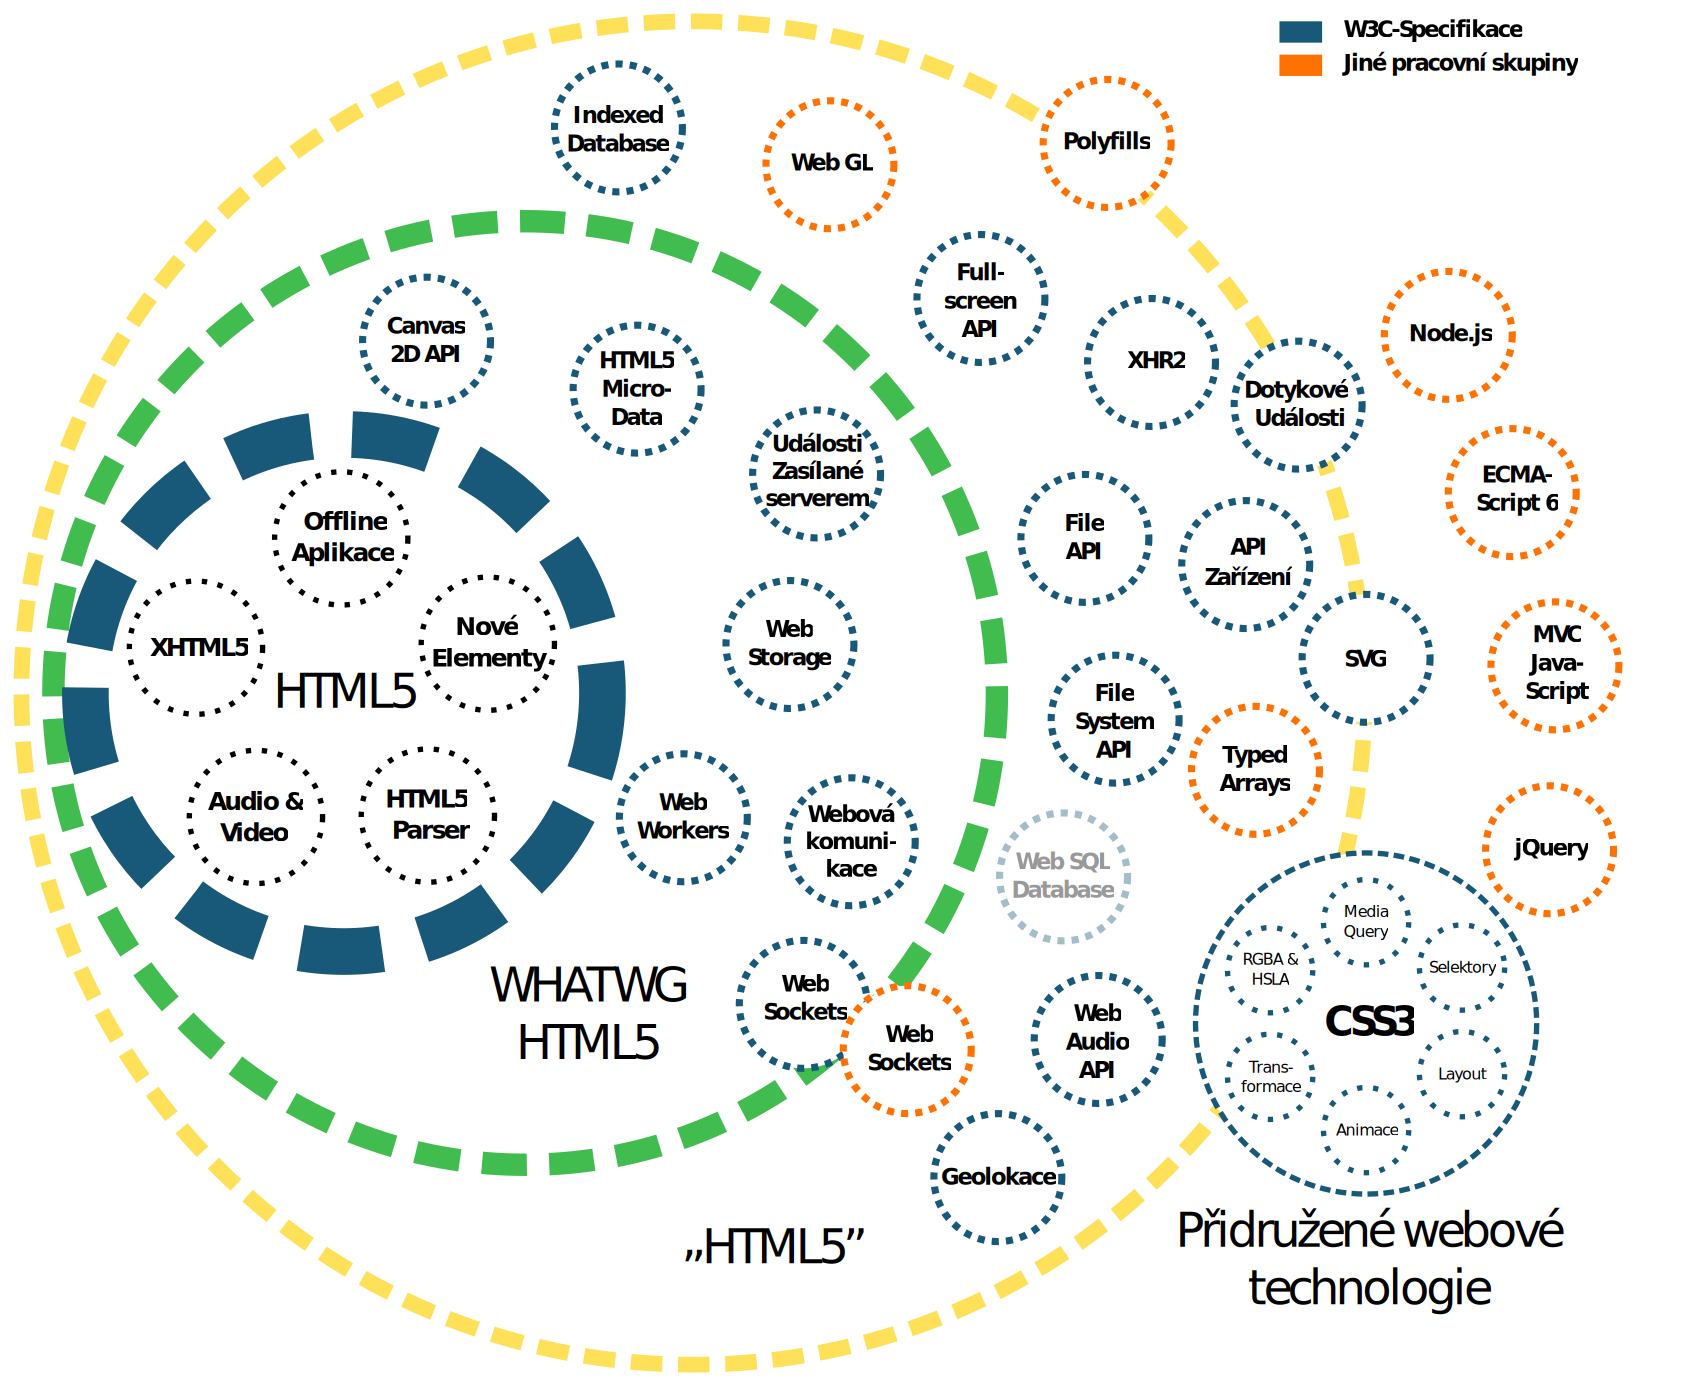
\includegraphics[width=1.0\textwidth]{html5api}
\caption{HTML 5 API}
\label{fig:html5api}
\end{figure}

\chapter{Diagram návrhu webu}
\begin{figure}[htb]
\centering
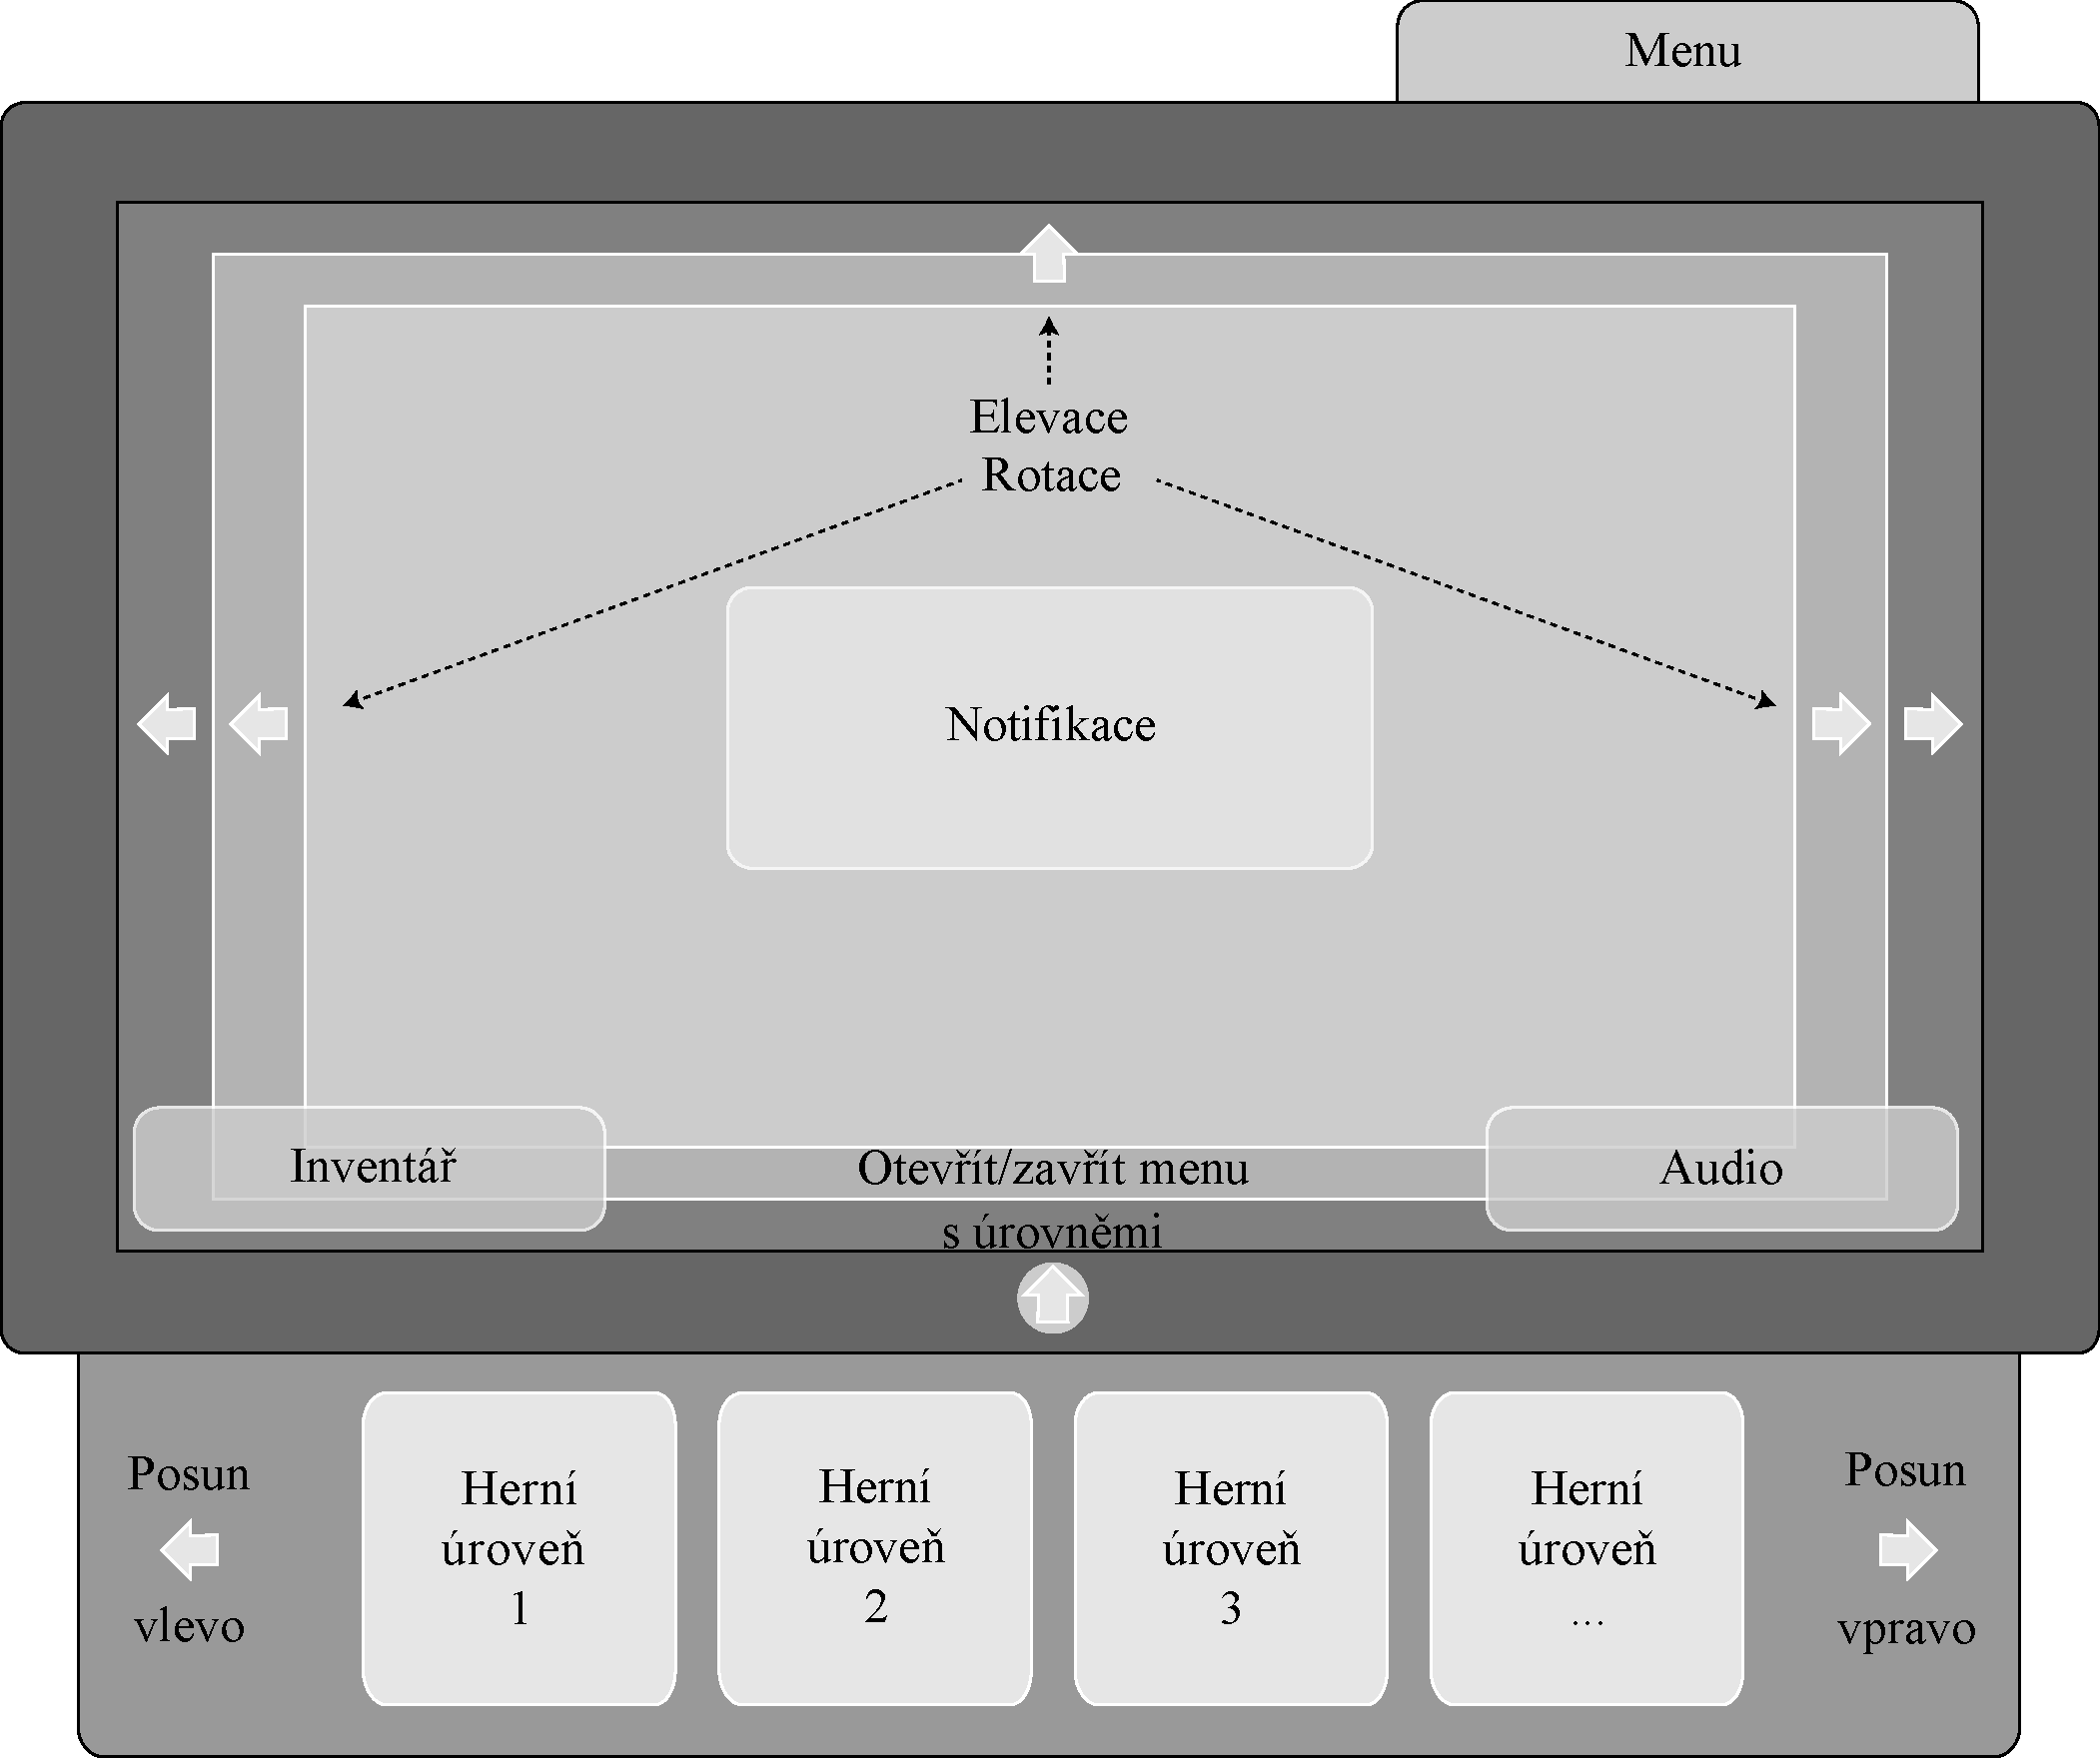
\includegraphics[width=1.0\textwidth]{web}
\caption{Návrh webu}
\label{fig:web}
\end{figure}

%\chapter{Diagram ovládání kamery}
%\begin{figure}[htb]
%\centering
%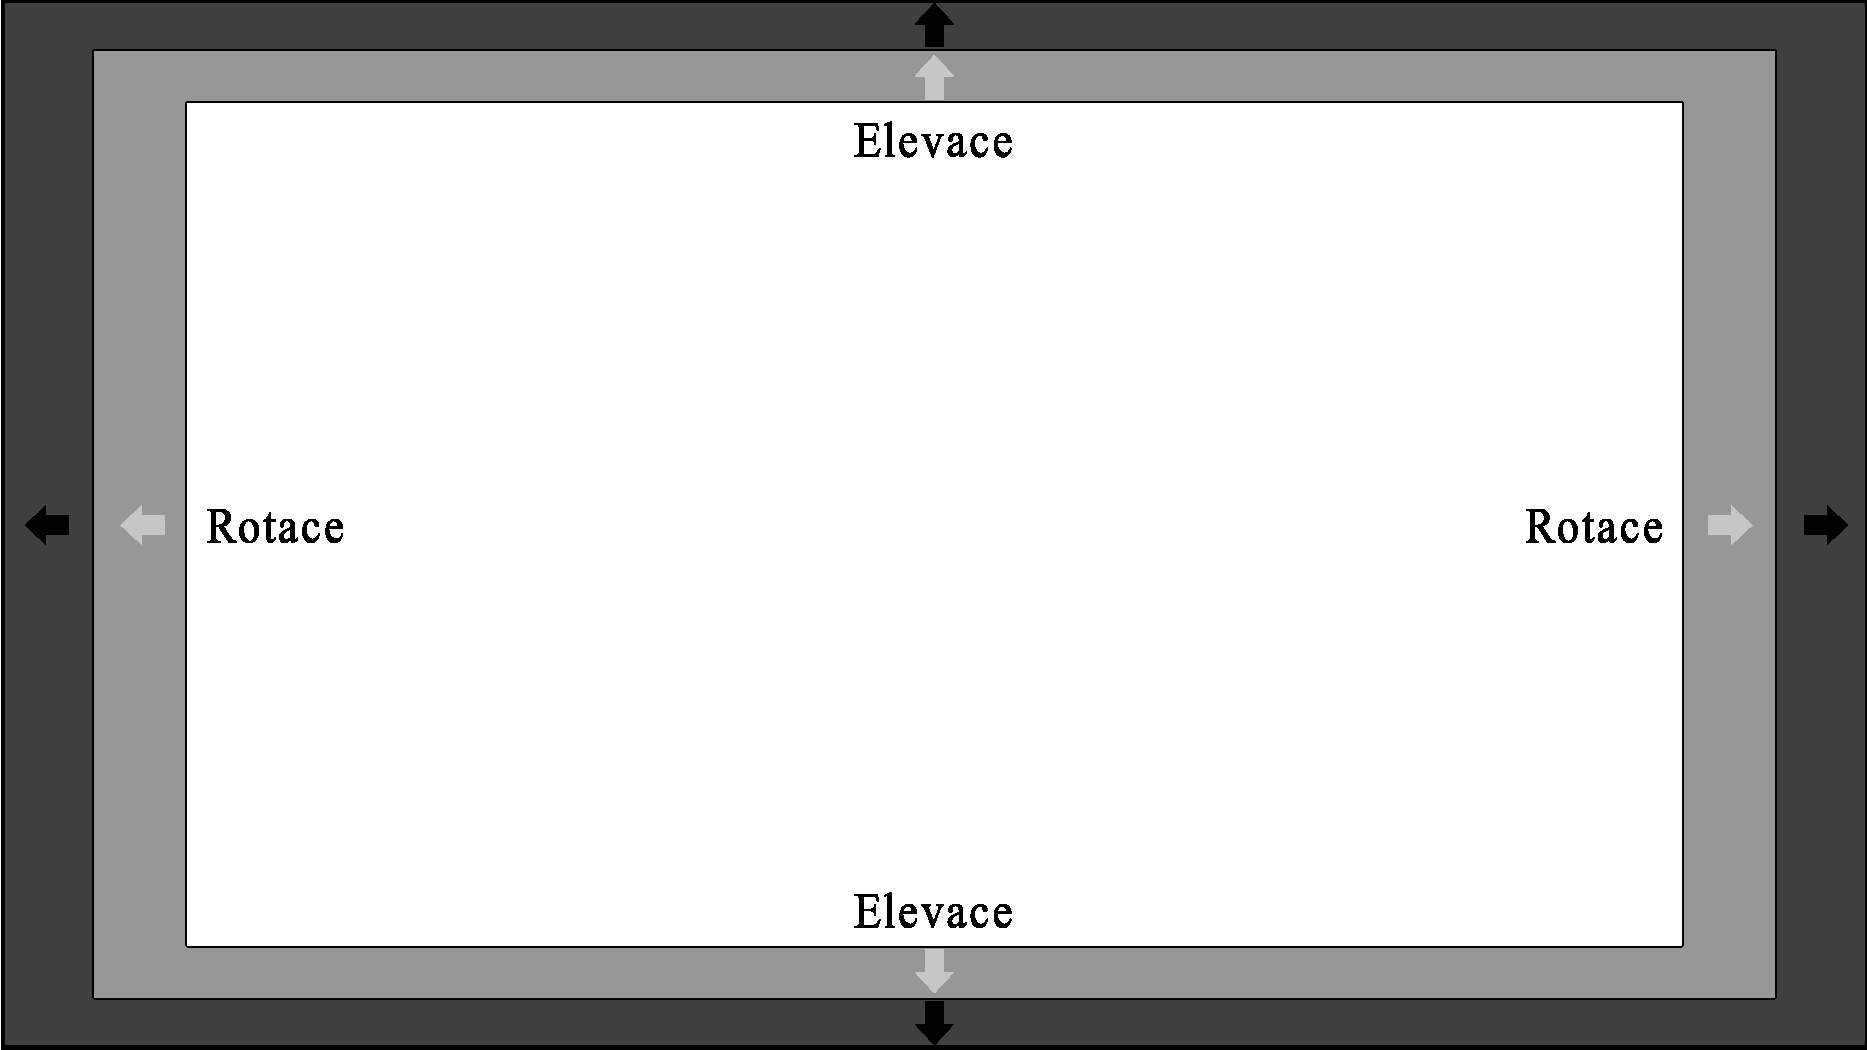
\includegraphics[width=1.0\textwidth]{mouseCamera}
%\caption{Ovládání kamery}
%\label{fig:mouseCamera}
%\end{figure}

\chapter{Podoba hry Berušky 2 WebGL}
\begin{figure}[htb]
\centering
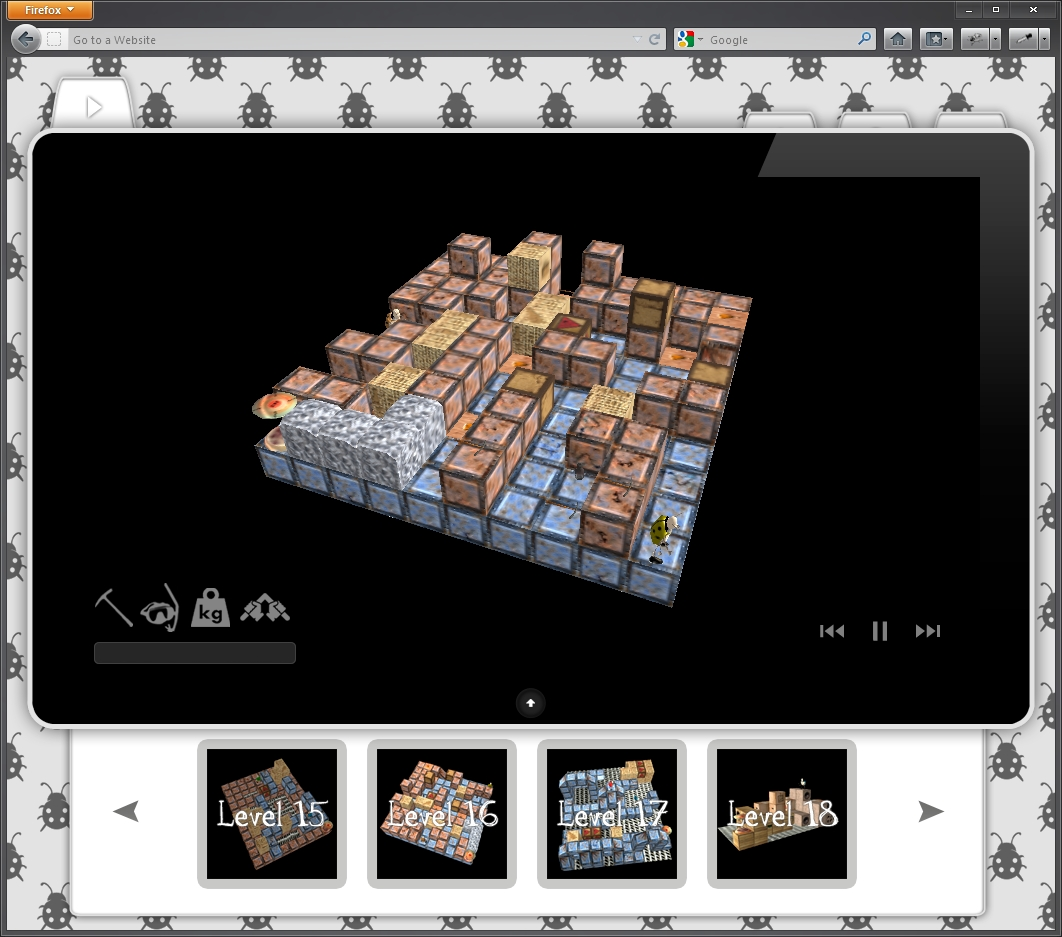
\includegraphics[width=1.0\textwidth]{bugEscapeWebGL}
\caption{Berušky 2 WebGL v prohlížeči Firefox 12}
\label{fig:gameImage}
\end{figure}

\chapter{Obsah DVD}
\begin{table}[!ht]
\label{table:dvd}
\begin{center}
\begin{tabular}{ | l | l |}
\hline
\textbf{Cesta} & \textbf{Popis} \\ \hline
\texttt{./audio} & Herní hudba \\ \hline
\texttt{./css} & Kaskádové styly \\ \hline
\texttt{./doc} & Zdrojové soubory této práce \\ \hline
\texttt{./dochtml} & Vygenerovaná HTML dokumentace \\ \hline
\texttt{./graphics} & Zdrojové soubory grafiky \\ \hline
\texttt{./img} & Webová grafika \\ \hline
\texttt{./js} & Implementace hry a soubory frameworků \\ \hline
\texttt{./levels} & JSON soubory herních úrovní \\ \hline
\texttt{./lightmaps} & Lightmapy \\ \hline
\texttt{./textures} & Textury \\ \hline
\textbf{\texttt{./index.html}} & HTML dokument hry s GLSL popisem shaderů \\ \hline
\end{tabular}
\end{center}
\caption{Obsah DVD}
\end{table}



 % viz. prilohy.tex
\end{document}
